
\section[{Graphs, Networks, and Trees}]{Graphs, Networks, and Trees}\label{GD}\par
Graphical representations are widely used for displaying relations among informational units because they help readers to visualize those relations and hence to understand them better. Two general types of graphical representations may be distinguished. \begin{itemize}
\item \textit{Graphs}, in the strictly mathematical sense, consist of points, often called \textit{nodes} or \textit{vertices}, and connections among them, called \textit{arcs}, or under certain conditions, \textit{edges}. Among the various types of graphs are \textit{networks} and \textit{trees}. Graphs generally and networks in particular are dealt with directly below. Trees are dealt with separately in sections \textit{\hyperref[GDTR]{19.2.\ Trees}} and \textit{\hyperref[GDAT]{19.3.\ Another Tree Notation}}.\footnote{The treatment here is largely based on the characterizations of graph types in \cite{GD-BIBL-1}}
\item \textit{Charts}, which typically plot data in two or more dimensions, including plots with orthogonal or radial axes, bar charts, pie charts, and the like. These can be described using the elements defined in the module for figures and graphics; see chapter \textit{\hyperref[FT]{14.\ Tables, Formulæ, Graphics and Notated Music}}.
\end{itemize} \par
Among the types of qualitative relations often represented by graphs are organizational hierarchies, flow charts, genealogies, semantic networks, transition networks, grammatical relations, tournament schedules, seating plans, and directions to people's houses. In developing recommendations for the encoding of graphs of various types, we have relied on their formal mathematical definitions and on the most common conventions for representing them visually. However, it must be emphasized that these recommendations do not provide for the full range of possible graphical representations, and deal only partially with questions of design, layout, and placement.
\subsection[{Graphs and Digraphs}]{Graphs and Digraphs}\label{GDGR}\par
Broadly speaking, graphs can be divided into two types: \textit{undirected} and \textit{directed}. An undirected graph is a set of \textit{nodes} (or \textit{vertices}) together with a set of pairs of those vertices, called \textit{arcs} or \textit{edges}. Each node in an arc of an undirected graph is said to be \textit{incident} with that arc, and the two vertices (nodes) which make up an arc are said to be \textit{adjacent}. An directed graph is like an undirected graph except that the arcs are \textit{ordered pairs} of nodes. In the case of directed graphs, the term \textit{edge} is not used; moreover, each arc in a directed graph is said to be \textit{adjacent from} the node from which the arc emanates, and \textit{adjacent to} the node to which the arc is directed. We use the element \hyperref[TEI.graph]{<graph>} to encode graphs as a whole, \hyperref[TEI.node]{<node>} to encode nodes or vertices, and \hyperref[TEI.arc]{<arc>} to encode arcs or edges; arcs can also be encoded by attributes on the \hyperref[TEI.node]{<node>} element. These elements have the following descriptions and attributes: 
\begin{sansreflist}
  
\item [\textbf{<graph>}] (graph) encodes a graph, which is a collection of nodes, and arcs which connect the nodes.
\item [\textbf{<node>}] (node) encodes a node, a possibly labeled point in a graph.
\item [\textbf{<arc>}] (arc) encodes an arc, the connection from one node to another in a graph.
\end{sansreflist}
\par
Before proceeding, some additional terminology may be helpful. We define a \textit{path} in a graph as a sequence of nodes n1, ..., nk such that there is an arc from each ni to ni+1 in the sequence. A \textit{cyclic path}, or \textit{cycle} is a path leading from a particular node back to itself. A graph that contains at least one cycle is said to be \textit{cyclic}; otherwise it is \textit{acyclic}. We say, finally, that a graph is \textit{connected} if there is a path from some node to every other node in the graph; any graph that is not connected is said to be \textit{disconnected}.\par
Here is an example of an undirected, cyclic disconnected graph, in which the nodes are annotated with three-letter codes for airports, and the arcs connecting the nodes are represented by horizontal and vertical lines, with 90 degree bends used simply to avoid having to draw diagonal lines.\par
 \noindent\includegraphics[width=0.7\textwidth,]{Images/graph1.jpg}\par
Next is a markup of the graph, using \hyperref[TEI.arc]{<arc>} elements to encode the arcs. \par\bgroup\index{graph=<graph>|exampleindex}\index{type=@type!<graph>|exampleindex}\index{order=@order!<graph>|exampleindex}\index{size=@size!<graph>|exampleindex}\index{label=<label>|exampleindex}\index{node=<node>|exampleindex}\index{degree=@degree!<node>|exampleindex}\index{label=<label>|exampleindex}\index{node=<node>|exampleindex}\index{degree=@degree!<node>|exampleindex}\index{label=<label>|exampleindex}\index{node=<node>|exampleindex}\index{degree=@degree!<node>|exampleindex}\index{label=<label>|exampleindex}\index{node=<node>|exampleindex}\index{degree=@degree!<node>|exampleindex}\index{label=<label>|exampleindex}\index{node=<node>|exampleindex}\index{degree=@degree!<node>|exampleindex}\index{label=<label>|exampleindex}\index{arc=<arc>|exampleindex}\index{from=@from!<arc>|exampleindex}\index{to=@to!<arc>|exampleindex}\index{arc=<arc>|exampleindex}\index{from=@from!<arc>|exampleindex}\index{to=@to!<arc>|exampleindex}\index{arc=<arc>|exampleindex}\index{from=@from!<arc>|exampleindex}\index{to=@to!<arc>|exampleindex}\index{arc=<arc>|exampleindex}\index{from=@from!<arc>|exampleindex}\index{to=@to!<arc>|exampleindex}\exampleFont \begin{shaded}\noindent\mbox{}{<\textbf{graph}\hspace*{1em}{type}="{undirected}"\hspace*{1em}{xml:id}="{CUG1}"\mbox{}\newline 
\hspace*{1em}{order}="{5}"\hspace*{1em}{size}="{4}">}\mbox{}\newline 
\hspace*{1em}{<\textbf{label}>}Airline Connections in Southwestern USA{</\textbf{label}>}\mbox{}\newline 
\hspace*{1em}{<\textbf{node}\hspace*{1em}{xml:id}="{LAX}"\hspace*{1em}{degree}="{2}">}\mbox{}\newline 
\hspace*{1em}\hspace*{1em}{<\textbf{label}>}LAX{</\textbf{label}>}\mbox{}\newline 
\hspace*{1em}{</\textbf{node}>}\mbox{}\newline 
\hspace*{1em}{<\textbf{node}\hspace*{1em}{xml:id}="{LVG}"\hspace*{1em}{degree}="{2}">}\mbox{}\newline 
\hspace*{1em}\hspace*{1em}{<\textbf{label}>}LVG{</\textbf{label}>}\mbox{}\newline 
\hspace*{1em}{</\textbf{node}>}\mbox{}\newline 
\hspace*{1em}{<\textbf{node}\hspace*{1em}{xml:id}="{PHX}"\hspace*{1em}{degree}="{3}">}\mbox{}\newline 
\hspace*{1em}\hspace*{1em}{<\textbf{label}>}PHX{</\textbf{label}>}\mbox{}\newline 
\hspace*{1em}{</\textbf{node}>}\mbox{}\newline 
\hspace*{1em}{<\textbf{node}\hspace*{1em}{xml:id}="{TUS}"\hspace*{1em}{degree}="{1}">}\mbox{}\newline 
\hspace*{1em}\hspace*{1em}{<\textbf{label}>}TUS{</\textbf{label}>}\mbox{}\newline 
\hspace*{1em}{</\textbf{node}>}\mbox{}\newline 
\hspace*{1em}{<\textbf{node}\hspace*{1em}{xml:id}="{CIB}"\hspace*{1em}{degree}="{0}">}\mbox{}\newline 
\hspace*{1em}\hspace*{1em}{<\textbf{label}>}CIB{</\textbf{label}>}\mbox{}\newline 
\hspace*{1em}{</\textbf{node}>}\mbox{}\newline 
\hspace*{1em}{<\textbf{arc}\hspace*{1em}{from}="{\#LAX}"\hspace*{1em}{to}="{\#LVG}"/>}\mbox{}\newline 
\hspace*{1em}{<\textbf{arc}\hspace*{1em}{from}="{\#LAX}"\hspace*{1em}{to}="{\#PHX}"/>}\mbox{}\newline 
\hspace*{1em}{<\textbf{arc}\hspace*{1em}{from}="{\#LVG}"\hspace*{1em}{to}="{\#PHX}"/>}\mbox{}\newline 
\hspace*{1em}{<\textbf{arc}\hspace*{1em}{from}="{\#PHX}"\hspace*{1em}{to}="{\#TUS}"/>}\mbox{}\newline 
{</\textbf{graph}>}\end{shaded}\egroup\par \par
The first child element of \hyperref[TEI.graph]{<graph>} may be a \hyperref[TEI.label]{<label>} to record a label for the graph; similarly, the \hyperref[TEI.label]{<label>} child of each \hyperref[TEI.node]{<node>} element records the labels of that node. The {\itshape order} and {\itshape size} attributes on the \hyperref[TEI.graph]{<graph>} element record the number of nodes and number of arcs in the graph respectively; these values are optional (since they can be computed from the rest of the graph), but if they are supplied, they must be consistent with the rest of the encoding. They can thus be used to help check that the graph has been encoded and transmitted correctly. The {\itshape degree} attribute on the \hyperref[TEI.node]{<node>} elements record the number of arcs that are incident with that node. It is optional (because redundant), but can be used to help in validity checking: if a value is given, it must be consistent with the rest of the information in the graph. Finally, the {\itshape from} and {\itshape to} attributes on the \hyperref[TEI.arc]{<arc>} elements provide pointers to the nodes connected by those arcs. Since the graph is undirected, no directionality is implied by the use of the {\itshape from} and {\itshape to} attributes; the values of these attributes could be interchanged in each arc without changing the graph.\par
The {\itshape adj}, {\itshape adjFrom}, and {\itshape adjTo} attributes of the \hyperref[TEI.node]{<node>} element provide an alternative method of representing unlabeled arcs, their values being pointers to the nodes which are adjacent to or from that node. The {\itshape adj} attribute is to be used for undirected graphs, and the {\itshape adjFrom} and {\itshape adjTo} attributes for directed graphs. It is a semantic error for the directed adjacency attributes to be used in an undirected graph, and vice versa. Here is a markup of the preceding graph, using the {\itshape adj} attribute to represent the arcs. \par\bgroup\index{graph=<graph>|exampleindex}\index{type=@type!<graph>|exampleindex}\index{order=@order!<graph>|exampleindex}\index{size=@size!<graph>|exampleindex}\index{label=<label>|exampleindex}\index{node=<node>|exampleindex}\index{degree=@degree!<node>|exampleindex}\index{adj=@adj!<node>|exampleindex}\index{label=<label>|exampleindex}\index{node=<node>|exampleindex}\index{degree=@degree!<node>|exampleindex}\index{adj=@adj!<node>|exampleindex}\index{label=<label>|exampleindex}\index{node=<node>|exampleindex}\index{degree=@degree!<node>|exampleindex}\index{adj=@adj!<node>|exampleindex}\index{label=<label>|exampleindex}\index{node=<node>|exampleindex}\index{degree=@degree!<node>|exampleindex}\index{adj=@adj!<node>|exampleindex}\index{label=<label>|exampleindex}\index{node=<node>|exampleindex}\index{degree=@degree!<node>|exampleindex}\index{label=<label>|exampleindex}\exampleFont \begin{shaded}\noindent\mbox{}{<\textbf{graph}\hspace*{1em}{type}="{undirected}"\hspace*{1em}{xml:id}="{CUG2}"\mbox{}\newline 
\hspace*{1em}{order}="{5}"\hspace*{1em}{size}="{4}">}\mbox{}\newline 
\hspace*{1em}{<\textbf{label}>}Airline Connections in Southwestern USA{</\textbf{label}>}\mbox{}\newline 
\hspace*{1em}{<\textbf{node}\hspace*{1em}{xml:id}="{LAX2}"\hspace*{1em}{degree}="{2}"\mbox{}\newline 
\hspace*{1em}\hspace*{1em}{adj}="{\#LVG2 \#PHX2}">}\mbox{}\newline 
\hspace*{1em}\hspace*{1em}{<\textbf{label}>}LAX2{</\textbf{label}>}\mbox{}\newline 
\hspace*{1em}{</\textbf{node}>}\mbox{}\newline 
\hspace*{1em}{<\textbf{node}\hspace*{1em}{xml:id}="{LVG2}"\hspace*{1em}{degree}="{2}"\mbox{}\newline 
\hspace*{1em}\hspace*{1em}{adj}="{\#LAX2 \#PHX2}">}\mbox{}\newline 
\hspace*{1em}\hspace*{1em}{<\textbf{label}>}LVG2{</\textbf{label}>}\mbox{}\newline 
\hspace*{1em}{</\textbf{node}>}\mbox{}\newline 
\hspace*{1em}{<\textbf{node}\hspace*{1em}{xml:id}="{PHX2}"\hspace*{1em}{degree}="{3}"\mbox{}\newline 
\hspace*{1em}\hspace*{1em}{adj}="{\#LAX2 \#LVG2 \#TUS2}">}\mbox{}\newline 
\hspace*{1em}\hspace*{1em}{<\textbf{label}>}PHX2{</\textbf{label}>}\mbox{}\newline 
\hspace*{1em}{</\textbf{node}>}\mbox{}\newline 
\hspace*{1em}{<\textbf{node}\hspace*{1em}{xml:id}="{TUS2}"\hspace*{1em}{degree}="{1}"\hspace*{1em}{adj}="{\#PHX2}">}\mbox{}\newline 
\hspace*{1em}\hspace*{1em}{<\textbf{label}>}TUS2{</\textbf{label}>}\mbox{}\newline 
\hspace*{1em}{</\textbf{node}>}\mbox{}\newline 
\hspace*{1em}{<\textbf{node}\hspace*{1em}{xml:id}="{CIB2}"\hspace*{1em}{degree}="{0}">}\mbox{}\newline 
\hspace*{1em}\hspace*{1em}{<\textbf{label}>}CIB2{</\textbf{label}>}\mbox{}\newline 
\hspace*{1em}{</\textbf{node}>}\mbox{}\newline 
{</\textbf{graph}>}\end{shaded}\egroup\par \par
Note that each arc is represented twice in this encoding of the graph. For example, the existence of the arc from LAX to LVG can be inferred from each of the first two \hyperref[TEI.node]{<node>} elements in the graph. This redundancy, however, is not required: it suffices to describe an arc in any one of the three places it can be described (either adjacent node, or in a separate \hyperref[TEI.arc]{<arc>} element). Here is a less redundant representation of the same graph. \par\bgroup\index{graph=<graph>|exampleindex}\index{type=@type!<graph>|exampleindex}\index{order=@order!<graph>|exampleindex}\index{size=@size!<graph>|exampleindex}\index{label=<label>|exampleindex}\index{node=<node>|exampleindex}\index{degree=@degree!<node>|exampleindex}\index{adj=@adj!<node>|exampleindex}\index{label=<label>|exampleindex}\index{node=<node>|exampleindex}\index{degree=@degree!<node>|exampleindex}\index{adj=@adj!<node>|exampleindex}\index{label=<label>|exampleindex}\index{node=<node>|exampleindex}\index{degree=@degree!<node>|exampleindex}\index{adj=@adj!<node>|exampleindex}\index{label=<label>|exampleindex}\index{node=<node>|exampleindex}\index{degree=@degree!<node>|exampleindex}\index{label=<label>|exampleindex}\index{node=<node>|exampleindex}\index{degree=@degree!<node>|exampleindex}\index{label=<label>|exampleindex}\exampleFont \begin{shaded}\noindent\mbox{}{<\textbf{graph}\hspace*{1em}{type}="{undirected}"\hspace*{1em}{xml:id}="{CUG3}"\mbox{}\newline 
\hspace*{1em}{order}="{5}"\hspace*{1em}{size}="{4}">}\mbox{}\newline 
\hspace*{1em}{<\textbf{label}>}Airline Connections in Southwestern USA{</\textbf{label}>}\mbox{}\newline 
\hspace*{1em}{<\textbf{node}\hspace*{1em}{xml:id}="{LAX3}"\hspace*{1em}{degree}="{2}"\mbox{}\newline 
\hspace*{1em}\hspace*{1em}{adj}="{\#LVG3 \#PHX3}">}\mbox{}\newline 
\hspace*{1em}\hspace*{1em}{<\textbf{label}>}LAX3{</\textbf{label}>}\mbox{}\newline 
\hspace*{1em}{</\textbf{node}>}\mbox{}\newline 
\hspace*{1em}{<\textbf{node}\hspace*{1em}{xml:id}="{LVG3}"\hspace*{1em}{degree}="{2}"\hspace*{1em}{adj}="{\#PHX3}">}\mbox{}\newline 
\hspace*{1em}\hspace*{1em}{<\textbf{label}>}LVG3{</\textbf{label}>}\mbox{}\newline 
\hspace*{1em}{</\textbf{node}>}\mbox{}\newline 
\hspace*{1em}{<\textbf{node}\hspace*{1em}{xml:id}="{PHX3}"\hspace*{1em}{degree}="{3}"\hspace*{1em}{adj}="{\#TUS3}">}\mbox{}\newline 
\hspace*{1em}\hspace*{1em}{<\textbf{label}>}PHX3{</\textbf{label}>}\mbox{}\newline 
\hspace*{1em}{</\textbf{node}>}\mbox{}\newline 
\hspace*{1em}{<\textbf{node}\hspace*{1em}{xml:id}="{TUS3}"\hspace*{1em}{degree}="{1}">}\mbox{}\newline 
\hspace*{1em}\hspace*{1em}{<\textbf{label}>}TUS3{</\textbf{label}>}\mbox{}\newline 
\hspace*{1em}{</\textbf{node}>}\mbox{}\newline 
\hspace*{1em}{<\textbf{node}\hspace*{1em}{xml:id}="{CIB3}"\hspace*{1em}{degree}="{0}">}\mbox{}\newline 
\hspace*{1em}\hspace*{1em}{<\textbf{label}>}CIB3{</\textbf{label}>}\mbox{}\newline 
\hspace*{1em}{</\textbf{node}>}\mbox{}\newline 
{</\textbf{graph}>}\end{shaded}\egroup\par \par
Although in many cases the \hyperref[TEI.arc]{<arc>} element is redundant (since arcs can be described using the adjacency attributes of their adjacent nodes), it has nevertheless been included in this module, in order to allow the convenient specification of identifiers, display or rendition information, and labels for each arc (using the attributes {\itshape xml:id}, {\itshape rend}, and a child \hyperref[TEI.label]{<label>} element).\par
Next, let us modify the preceding graph by adding directionality to the arcs. Specifically, we now think of the arcs as specifying selected routes from one airport to another, as indicated by the direction of the arrowheads in the following diagram.\par
 \noindent\includegraphics[width=0.7\textwidth,]{Images/graph2.jpg}\par
Here is an encoding of this graph, using the \hyperref[TEI.arc]{<arc>} element to designate the arcs. \par\bgroup\index{graph=<graph>|exampleindex}\index{type=@type!<graph>|exampleindex}\index{order=@order!<graph>|exampleindex}\index{size=@size!<graph>|exampleindex}\index{label=<label>|exampleindex}\index{node=<node>|exampleindex}\index{inDegree=@inDegree!<node>|exampleindex}\index{outDegree=@outDegree!<node>|exampleindex}\index{label=<label>|exampleindex}\index{node=<node>|exampleindex}\index{inDegree=@inDegree!<node>|exampleindex}\index{outDegree=@outDegree!<node>|exampleindex}\index{label=<label>|exampleindex}\index{node=<node>|exampleindex}\index{inDegree=@inDegree!<node>|exampleindex}\index{outDegree=@outDegree!<node>|exampleindex}\index{label=<label>|exampleindex}\index{node=<node>|exampleindex}\index{inDegree=@inDegree!<node>|exampleindex}\index{outDegree=@outDegree!<node>|exampleindex}\index{label=<label>|exampleindex}\index{node=<node>|exampleindex}\index{inDegree=@inDegree!<node>|exampleindex}\index{outDegree=@outDegree!<node>|exampleindex}\index{label=<label>|exampleindex}\index{arc=<arc>|exampleindex}\index{from=@from!<arc>|exampleindex}\index{to=@to!<arc>|exampleindex}\index{arc=<arc>|exampleindex}\index{from=@from!<arc>|exampleindex}\index{to=@to!<arc>|exampleindex}\index{arc=<arc>|exampleindex}\index{from=@from!<arc>|exampleindex}\index{to=@to!<arc>|exampleindex}\index{arc=<arc>|exampleindex}\index{from=@from!<arc>|exampleindex}\index{to=@to!<arc>|exampleindex}\index{arc=<arc>|exampleindex}\index{from=@from!<arc>|exampleindex}\index{to=@to!<arc>|exampleindex}\exampleFont \begin{shaded}\noindent\mbox{}{<\textbf{graph}\hspace*{1em}{type}="{directed}"\hspace*{1em}{xml:id}="{RDG1}"\mbox{}\newline 
\hspace*{1em}{order}="{5}"\hspace*{1em}{size}="{5}">}\mbox{}\newline 
\hspace*{1em}{<\textbf{label}>}Selected Airline Routes in Southwestern USA{</\textbf{label}>}\mbox{}\newline 
\hspace*{1em}{<\textbf{node}\hspace*{1em}{xml:id}="{LAX4}"\hspace*{1em}{inDegree}="{1}"\mbox{}\newline 
\hspace*{1em}\hspace*{1em}{outDegree}="{1}">}\mbox{}\newline 
\hspace*{1em}\hspace*{1em}{<\textbf{label}>}LAX4{</\textbf{label}>}\mbox{}\newline 
\hspace*{1em}{</\textbf{node}>}\mbox{}\newline 
\hspace*{1em}{<\textbf{node}\hspace*{1em}{xml:id}="{LVG4}"\hspace*{1em}{inDegree}="{1}"\mbox{}\newline 
\hspace*{1em}\hspace*{1em}{outDegree}="{1}">}\mbox{}\newline 
\hspace*{1em}\hspace*{1em}{<\textbf{label}>}LVG4{</\textbf{label}>}\mbox{}\newline 
\hspace*{1em}{</\textbf{node}>}\mbox{}\newline 
\hspace*{1em}{<\textbf{node}\hspace*{1em}{xml:id}="{PHX4}"\hspace*{1em}{inDegree}="{2}"\mbox{}\newline 
\hspace*{1em}\hspace*{1em}{outDegree}="{2}">}\mbox{}\newline 
\hspace*{1em}\hspace*{1em}{<\textbf{label}>}PHX4{</\textbf{label}>}\mbox{}\newline 
\hspace*{1em}{</\textbf{node}>}\mbox{}\newline 
\hspace*{1em}{<\textbf{node}\hspace*{1em}{xml:id}="{TUS4}"\hspace*{1em}{inDegree}="{1}"\mbox{}\newline 
\hspace*{1em}\hspace*{1em}{outDegree}="{1}">}\mbox{}\newline 
\hspace*{1em}\hspace*{1em}{<\textbf{label}>}TUS4{</\textbf{label}>}\mbox{}\newline 
\hspace*{1em}{</\textbf{node}>}\mbox{}\newline 
\hspace*{1em}{<\textbf{node}\hspace*{1em}{xml:id}="{CIB4}"\hspace*{1em}{inDegree}="{0}"\mbox{}\newline 
\hspace*{1em}\hspace*{1em}{outDegree}="{0}">}\mbox{}\newline 
\hspace*{1em}\hspace*{1em}{<\textbf{label}>}CIB4{</\textbf{label}>}\mbox{}\newline 
\hspace*{1em}{</\textbf{node}>}\mbox{}\newline 
\hspace*{1em}{<\textbf{arc}\hspace*{1em}{from}="{\#LAX4}"\hspace*{1em}{to}="{\#LVG4}"/>}\mbox{}\newline 
\hspace*{1em}{<\textbf{arc}\hspace*{1em}{from}="{\#LVG4}"\hspace*{1em}{to}="{\#PHX4}"/>}\mbox{}\newline 
\hspace*{1em}{<\textbf{arc}\hspace*{1em}{from}="{\#PHX4}"\hspace*{1em}{to}="{\#LAX4}"/>}\mbox{}\newline 
\hspace*{1em}{<\textbf{arc}\hspace*{1em}{from}="{\#PHX4}"\hspace*{1em}{to}="{\#TUS4}"/>}\mbox{}\newline 
\hspace*{1em}{<\textbf{arc}\hspace*{1em}{from}="{\#TUS4}"\hspace*{1em}{to}="{\#PHX4}"/>}\mbox{}\newline 
{</\textbf{graph}>}\end{shaded}\egroup\par \noindent  The attributes {\itshape inDegree} and {\itshape outDegree} indicate the number of nodes which are adjacent to and from the node concerned respectively.\par
Here is another encoding of the graph, using the {\itshape adjTo} and {\itshape adjFrom} attributes on nodes to designate the arcs. \par\bgroup\index{graph=<graph>|exampleindex}\index{type=@type!<graph>|exampleindex}\index{order=@order!<graph>|exampleindex}\index{size=@size!<graph>|exampleindex}\index{label=<label>|exampleindex}\index{node=<node>|exampleindex}\index{inDegree=@inDegree!<node>|exampleindex}\index{outDegree=@outDegree!<node>|exampleindex}\index{adjTo=@adjTo!<node>|exampleindex}\index{adjFrom=@adjFrom!<node>|exampleindex}\index{label=<label>|exampleindex}\index{node=<node>|exampleindex}\index{inDegree=@inDegree!<node>|exampleindex}\index{outDegree=@outDegree!<node>|exampleindex}\index{adjFrom=@adjFrom!<node>|exampleindex}\index{adjTo=@adjTo!<node>|exampleindex}\index{label=<label>|exampleindex}\index{node=<node>|exampleindex}\index{inDegree=@inDegree!<node>|exampleindex}\index{outDegree=@outDegree!<node>|exampleindex}\index{adjTo=@adjTo!<node>|exampleindex}\index{adjFrom=@adjFrom!<node>|exampleindex}\index{label=<label>|exampleindex}\index{node=<node>|exampleindex}\index{inDegree=@inDegree!<node>|exampleindex}\index{outDegree=@outDegree!<node>|exampleindex}\index{adjTo=@adjTo!<node>|exampleindex}\index{adjFrom=@adjFrom!<node>|exampleindex}\index{label=<label>|exampleindex}\index{node=<node>|exampleindex}\index{inDegree=@inDegree!<node>|exampleindex}\index{outDegree=@outDegree!<node>|exampleindex}\index{label=<label>|exampleindex}\exampleFont \begin{shaded}\noindent\mbox{}{<\textbf{graph}\hspace*{1em}{type}="{directed}"\hspace*{1em}{xml:id}="{RDG2}"\mbox{}\newline 
\hspace*{1em}{order}="{5}"\hspace*{1em}{size}="{5}">}\mbox{}\newline 
\hspace*{1em}{<\textbf{label}>}Selected Airline Routes in Southwestern USA{</\textbf{label}>}\mbox{}\newline 
\hspace*{1em}{<\textbf{node}\hspace*{1em}{xml:id}="{LAX5}"\hspace*{1em}{inDegree}="{1}"\mbox{}\newline 
\hspace*{1em}\hspace*{1em}{outDegree}="{1}"\hspace*{1em}{adjTo}="{\#LVG5}"\hspace*{1em}{adjFrom}="{\#PHX5}">}\mbox{}\newline 
\hspace*{1em}\hspace*{1em}{<\textbf{label}>}LAX5{</\textbf{label}>}\mbox{}\newline 
\hspace*{1em}{</\textbf{node}>}\mbox{}\newline 
\hspace*{1em}{<\textbf{node}\hspace*{1em}{xml:id}="{LVG5}"\hspace*{1em}{inDegree}="{1}"\mbox{}\newline 
\hspace*{1em}\hspace*{1em}{outDegree}="{1}"\hspace*{1em}{adjFrom}="{\#LAX5}"\hspace*{1em}{adjTo}="{\#PHX5}">}\mbox{}\newline 
\hspace*{1em}\hspace*{1em}{<\textbf{label}>}LVG5{</\textbf{label}>}\mbox{}\newline 
\hspace*{1em}{</\textbf{node}>}\mbox{}\newline 
\hspace*{1em}{<\textbf{node}\hspace*{1em}{xml:id}="{PHX5}"\hspace*{1em}{inDegree}="{2}"\mbox{}\newline 
\hspace*{1em}\hspace*{1em}{outDegree}="{2}"\hspace*{1em}{adjTo}="{\#LAX5 \#TUS}"\hspace*{1em}{adjFrom}="{\#LVG5 \#TUS5}">}\mbox{}\newline 
\hspace*{1em}\hspace*{1em}{<\textbf{label}>}PHX5{</\textbf{label}>}\mbox{}\newline 
\hspace*{1em}{</\textbf{node}>}\mbox{}\newline 
\hspace*{1em}{<\textbf{node}\hspace*{1em}{xml:id}="{TUS5}"\hspace*{1em}{inDegree}="{1}"\mbox{}\newline 
\hspace*{1em}\hspace*{1em}{outDegree}="{1}"\hspace*{1em}{adjTo}="{\#PHX5}"\hspace*{1em}{adjFrom}="{\#PHX5}">}\mbox{}\newline 
\hspace*{1em}\hspace*{1em}{<\textbf{label}>}TUS5{</\textbf{label}>}\mbox{}\newline 
\hspace*{1em}{</\textbf{node}>}\mbox{}\newline 
\hspace*{1em}{<\textbf{node}\hspace*{1em}{xml:id}="{CIB5}"\hspace*{1em}{inDegree}="{0}"\mbox{}\newline 
\hspace*{1em}\hspace*{1em}{outDegree}="{0}">}\mbox{}\newline 
\hspace*{1em}\hspace*{1em}{<\textbf{label}>}CIB5{</\textbf{label}>}\mbox{}\newline 
\hspace*{1em}{</\textbf{node}>}\mbox{}\newline 
{</\textbf{graph}>}\end{shaded}\egroup\par \par
If we wish to label the arcs, say with flight numbers, then \hyperref[TEI.arc]{<arc>} elements must be used to hold the \hyperref[TEI.label]{<label>} elements, as in the following example. \par\bgroup\index{graph=<graph>|exampleindex}\index{type=@type!<graph>|exampleindex}\index{order=@order!<graph>|exampleindex}\index{size=@size!<graph>|exampleindex}\index{label=<label>|exampleindex}\index{node=<node>|exampleindex}\index{label=<label>|exampleindex}\index{node=<node>|exampleindex}\index{label=<label>|exampleindex}\index{node=<node>|exampleindex}\index{label=<label>|exampleindex}\index{node=<node>|exampleindex}\index{label=<label>|exampleindex}\index{node=<node>|exampleindex}\index{label=<label>|exampleindex}\index{arc=<arc>|exampleindex}\index{from=@from!<arc>|exampleindex}\index{to=@to!<arc>|exampleindex}\index{label=<label>|exampleindex}\index{arc=<arc>|exampleindex}\index{from=@from!<arc>|exampleindex}\index{to=@to!<arc>|exampleindex}\index{label=<label>|exampleindex}\index{arc=<arc>|exampleindex}\index{from=@from!<arc>|exampleindex}\index{to=@to!<arc>|exampleindex}\index{label=<label>|exampleindex}\index{arc=<arc>|exampleindex}\index{from=@from!<arc>|exampleindex}\index{to=@to!<arc>|exampleindex}\index{label=<label>|exampleindex}\index{arc=<arc>|exampleindex}\index{from=@from!<arc>|exampleindex}\index{to=@to!<arc>|exampleindex}\index{label=<label>|exampleindex}\exampleFont \begin{shaded}\noindent\mbox{}{<\textbf{graph}\hspace*{1em}{type}="{directed}"\hspace*{1em}{xml:id}="{RDG3}"\mbox{}\newline 
\hspace*{1em}{order}="{5}"\hspace*{1em}{size}="{5}">}\mbox{}\newline 
\hspace*{1em}{<\textbf{label}>}Selected Airline Routes in Southwestern USA{</\textbf{label}>}\mbox{}\newline 
\hspace*{1em}{<\textbf{node}\hspace*{1em}{xml:id}="{LAX6}">}\mbox{}\newline 
\hspace*{1em}\hspace*{1em}{<\textbf{label}>}LAX6{</\textbf{label}>}\mbox{}\newline 
\hspace*{1em}{</\textbf{node}>}\mbox{}\newline 
\hspace*{1em}{<\textbf{node}\hspace*{1em}{xml:id}="{LVG6}">}\mbox{}\newline 
\hspace*{1em}\hspace*{1em}{<\textbf{label}>}LVG6{</\textbf{label}>}\mbox{}\newline 
\hspace*{1em}{</\textbf{node}>}\mbox{}\newline 
\hspace*{1em}{<\textbf{node}\hspace*{1em}{xml:id}="{PHX6}">}\mbox{}\newline 
\hspace*{1em}\hspace*{1em}{<\textbf{label}>}PHX6{</\textbf{label}>}\mbox{}\newline 
\hspace*{1em}{</\textbf{node}>}\mbox{}\newline 
\hspace*{1em}{<\textbf{node}\hspace*{1em}{xml:id}="{TUS6}">}\mbox{}\newline 
\hspace*{1em}\hspace*{1em}{<\textbf{label}>}TUS6{</\textbf{label}>}\mbox{}\newline 
\hspace*{1em}{</\textbf{node}>}\mbox{}\newline 
\hspace*{1em}{<\textbf{node}\hspace*{1em}{xml:id}="{CIB6}">}\mbox{}\newline 
\hspace*{1em}\hspace*{1em}{<\textbf{label}>}CIB6{</\textbf{label}>}\mbox{}\newline 
\hspace*{1em}{</\textbf{node}>}\mbox{}\newline 
\hspace*{1em}{<\textbf{arc}\hspace*{1em}{from}="{\#LAX6}"\hspace*{1em}{to}="{\#LVG6}">}\mbox{}\newline 
\hspace*{1em}\hspace*{1em}{<\textbf{label}>}SW117{</\textbf{label}>}\mbox{}\newline 
\hspace*{1em}{</\textbf{arc}>}\mbox{}\newline 
\hspace*{1em}{<\textbf{arc}\hspace*{1em}{from}="{\#LVG6}"\hspace*{1em}{to}="{\#PHX6}">}\mbox{}\newline 
\hspace*{1em}\hspace*{1em}{<\textbf{label}>}SW711{</\textbf{label}>}\mbox{}\newline 
\hspace*{1em}{</\textbf{arc}>}\mbox{}\newline 
\hspace*{1em}{<\textbf{arc}\hspace*{1em}{from}="{\#PHX6}"\hspace*{1em}{to}="{\#LAX6}">}\mbox{}\newline 
\hspace*{1em}\hspace*{1em}{<\textbf{label}>}AA218{</\textbf{label}>}\mbox{}\newline 
\hspace*{1em}{</\textbf{arc}>}\mbox{}\newline 
\hspace*{1em}{<\textbf{arc}\hspace*{1em}{from}="{\#PHX6}"\hspace*{1em}{to}="{\#TUS6}">}\mbox{}\newline 
\hspace*{1em}\hspace*{1em}{<\textbf{label}>}AW229{</\textbf{label}>}\mbox{}\newline 
\hspace*{1em}{</\textbf{arc}>}\mbox{}\newline 
\hspace*{1em}{<\textbf{arc}\hspace*{1em}{from}="{\#TUS6}"\hspace*{1em}{to}="{\#PHX6}">}\mbox{}\newline 
\hspace*{1em}\hspace*{1em}{<\textbf{label}>}AW225{</\textbf{label}>}\mbox{}\newline 
\hspace*{1em}{</\textbf{arc}>}\mbox{}\newline 
{</\textbf{graph}>}\end{shaded}\egroup\par \noindent  
\subsubsection[{Transition Networks}]{Transition Networks}\label{GDTN}\par
For encoding transition networks and other kinds of directed graphs in which distinctions among types of nodes must be made, the {\itshape type} attribute is provided for \hyperref[TEI.node]{<node>} elements. In the following example, the \textit{initial} and \textit{final} nodes (or \textit{states}) of the network are distinguished. It can be understood as accepting the set of strings obtained by traversing it from its initial node to its final node, and concatenating the labels. \par
 \noindent\includegraphics[width=0.6\textwidth,]{Images/graph3.jpg} \par\bgroup\index{graph=<graph>|exampleindex}\index{type=@type!<graph>|exampleindex}\index{order=@order!<graph>|exampleindex}\index{size=@size!<graph>|exampleindex}\index{label=<label>|exampleindex}\index{node=<node>|exampleindex}\index{inDegree=@inDegree!<node>|exampleindex}\index{outDegree=@outDegree!<node>|exampleindex}\index{type=@type!<node>|exampleindex}\index{node=<node>|exampleindex}\index{inDegree=@inDegree!<node>|exampleindex}\index{outDegree=@outDegree!<node>|exampleindex}\index{node=<node>|exampleindex}\index{inDegree=@inDegree!<node>|exampleindex}\index{outDegree=@outDegree!<node>|exampleindex}\index{node=<node>|exampleindex}\index{inDegree=@inDegree!<node>|exampleindex}\index{outDegree=@outDegree!<node>|exampleindex}\index{node=<node>|exampleindex}\index{inDegree=@inDegree!<node>|exampleindex}\index{outDegree=@outDegree!<node>|exampleindex}\index{type=@type!<node>|exampleindex}\index{arc=<arc>|exampleindex}\index{from=@from!<arc>|exampleindex}\index{to=@to!<arc>|exampleindex}\index{label=<label>|exampleindex}\index{arc=<arc>|exampleindex}\index{from=@from!<arc>|exampleindex}\index{to=@to!<arc>|exampleindex}\index{label=<label>|exampleindex}\index{arc=<arc>|exampleindex}\index{from=@from!<arc>|exampleindex}\index{to=@to!<arc>|exampleindex}\index{label=<label>|exampleindex}\index{arc=<arc>|exampleindex}\index{from=@from!<arc>|exampleindex}\index{to=@to!<arc>|exampleindex}\index{label=<label>|exampleindex}\index{arc=<arc>|exampleindex}\index{from=@from!<arc>|exampleindex}\index{to=@to!<arc>|exampleindex}\index{label=<label>|exampleindex}\index{arc=<arc>|exampleindex}\index{from=@from!<arc>|exampleindex}\index{to=@to!<arc>|exampleindex}\index{label=<label>|exampleindex}\exampleFont \begin{shaded}\noindent\mbox{}{<\textbf{graph}\hspace*{1em}{type}="{network-transition}"\mbox{}\newline 
\hspace*{1em}{xml:id}="{SS8}"\hspace*{1em}{order}="{5}"\hspace*{1em}{size}="{6}">}\mbox{}\newline 
\hspace*{1em}{<\textbf{label}>}(8){</\textbf{label}>}\mbox{}\newline 
\hspace*{1em}{<\textbf{node}\hspace*{1em}{xml:id}="{Q0}"\hspace*{1em}{inDegree}="{0}"\mbox{}\newline 
\hspace*{1em}\hspace*{1em}{outDegree}="{1}"\hspace*{1em}{type}="{initial}"/>}\mbox{}\newline 
\hspace*{1em}{<\textbf{node}\hspace*{1em}{xml:id}="{Q1}"\hspace*{1em}{inDegree}="{2}"\mbox{}\newline 
\hspace*{1em}\hspace*{1em}{outDegree}="{3}"/>}\mbox{}\newline 
\hspace*{1em}{<\textbf{node}\hspace*{1em}{xml:id}="{Q2}"\hspace*{1em}{inDegree}="{1}"\mbox{}\newline 
\hspace*{1em}\hspace*{1em}{outDegree}="{1}"/>}\mbox{}\newline 
\hspace*{1em}{<\textbf{node}\hspace*{1em}{xml:id}="{Q3}"\hspace*{1em}{inDegree}="{1}"\mbox{}\newline 
\hspace*{1em}\hspace*{1em}{outDegree}="{1}"/>}\mbox{}\newline 
\hspace*{1em}{<\textbf{node}\hspace*{1em}{xml:id}="{Q4}"\hspace*{1em}{inDegree}="{2}"\mbox{}\newline 
\hspace*{1em}\hspace*{1em}{outDegree}="{0}"\hspace*{1em}{type}="{final}"/>}\mbox{}\newline 
\hspace*{1em}{<\textbf{arc}\hspace*{1em}{from}="{\#Q0}"\hspace*{1em}{to}="{\#Q1}">}\mbox{}\newline 
\hspace*{1em}\hspace*{1em}{<\textbf{label}>}THE{</\textbf{label}>}\mbox{}\newline 
\hspace*{1em}{</\textbf{arc}>}\mbox{}\newline 
\hspace*{1em}{<\textbf{arc}\hspace*{1em}{from}="{\#Q1}"\hspace*{1em}{to}="{\#Q1}">}\mbox{}\newline 
\hspace*{1em}\hspace*{1em}{<\textbf{label}>}OLD{</\textbf{label}>}\mbox{}\newline 
\hspace*{1em}{</\textbf{arc}>}\mbox{}\newline 
\hspace*{1em}{<\textbf{arc}\hspace*{1em}{from}="{\#Q1}"\hspace*{1em}{to}="{\#Q2}">}\mbox{}\newline 
\hspace*{1em}\hspace*{1em}{<\textbf{label}>}MAN{</\textbf{label}>}\mbox{}\newline 
\hspace*{1em}{</\textbf{arc}>}\mbox{}\newline 
\hspace*{1em}{<\textbf{arc}\hspace*{1em}{from}="{\#Q1}"\hspace*{1em}{to}="{\#Q3}">}\mbox{}\newline 
\hspace*{1em}\hspace*{1em}{<\textbf{label}>}MEN{</\textbf{label}>}\mbox{}\newline 
\hspace*{1em}{</\textbf{arc}>}\mbox{}\newline 
\hspace*{1em}{<\textbf{arc}\hspace*{1em}{from}="{\#Q2}"\hspace*{1em}{to}="{\#Q4}">}\mbox{}\newline 
\hspace*{1em}\hspace*{1em}{<\textbf{label}>}COMES{</\textbf{label}>}\mbox{}\newline 
\hspace*{1em}{</\textbf{arc}>}\mbox{}\newline 
\hspace*{1em}{<\textbf{arc}\hspace*{1em}{from}="{\#Q3}"\hspace*{1em}{to}="{\#Q4}">}\mbox{}\newline 
\hspace*{1em}\hspace*{1em}{<\textbf{label}>}COME{</\textbf{label}>}\mbox{}\newline 
\hspace*{1em}{</\textbf{arc}>}\mbox{}\newline 
{</\textbf{graph}>}\end{shaded}\egroup\par \par
A finite state transducer has two labels on each arc, and can be thought of as representing a mapping from one sequence of labels to the other. The following example represents a transducer for translating the English strings accepted by the network in the preceding example into French. The nodes have been annotated with numbers, for convenience.\par
 \noindent\includegraphics[width=0.6\textwidth,]{Images/graph4.jpg} \par\bgroup\index{graph=<graph>|exampleindex}\index{type=@type!<graph>|exampleindex}\index{order=@order!<graph>|exampleindex}\index{size=@size!<graph>|exampleindex}\index{node=<node>|exampleindex}\index{inDegree=@inDegree!<node>|exampleindex}\index{outDegree=@outDegree!<node>|exampleindex}\index{type=@type!<node>|exampleindex}\index{label=<label>|exampleindex}\index{node=<node>|exampleindex}\index{inDegree=@inDegree!<node>|exampleindex}\index{outDegree=@outDegree!<node>|exampleindex}\index{label=<label>|exampleindex}\index{node=<node>|exampleindex}\index{inDegree=@inDegree!<node>|exampleindex}\index{outDegree=@outDegree!<node>|exampleindex}\index{label=<label>|exampleindex}\index{node=<node>|exampleindex}\index{inDegree=@inDegree!<node>|exampleindex}\index{outDegree=@outDegree!<node>|exampleindex}\index{label=<label>|exampleindex}\index{node=<node>|exampleindex}\index{inDegree=@inDegree!<node>|exampleindex}\index{outDegree=@outDegree!<node>|exampleindex}\index{label=<label>|exampleindex}\index{node=<node>|exampleindex}\index{inDegree=@inDegree!<node>|exampleindex}\index{outDegree=@outDegree!<node>|exampleindex}\index{label=<label>|exampleindex}\index{node=<node>|exampleindex}\index{inDegree=@inDegree!<node>|exampleindex}\index{outDegree=@outDegree!<node>|exampleindex}\index{type=@type!<node>|exampleindex}\index{label=<label>|exampleindex}\index{arc=<arc>|exampleindex}\index{from=@from!<arc>|exampleindex}\index{to=@to!<arc>|exampleindex}\index{label=<label>|exampleindex}\index{label=<label>|exampleindex}\index{arc=<arc>|exampleindex}\index{from=@from!<arc>|exampleindex}\index{to=@to!<arc>|exampleindex}\index{label=<label>|exampleindex}\index{label=<label>|exampleindex}\index{arc=<arc>|exampleindex}\index{from=@from!<arc>|exampleindex}\index{to=@to!<arc>|exampleindex}\index{label=<label>|exampleindex}\index{label=<label>|exampleindex}\index{arc=<arc>|exampleindex}\index{from=@from!<arc>|exampleindex}\index{to=@to!<arc>|exampleindex}\index{label=<label>|exampleindex}\index{label=<label>|exampleindex}\index{arc=<arc>|exampleindex}\index{from=@from!<arc>|exampleindex}\index{to=@to!<arc>|exampleindex}\index{label=<label>|exampleindex}\index{label=<label>|exampleindex}\index{arc=<arc>|exampleindex}\index{from=@from!<arc>|exampleindex}\index{to=@to!<arc>|exampleindex}\index{label=<label>|exampleindex}\index{label=<label>|exampleindex}\index{arc=<arc>|exampleindex}\index{from=@from!<arc>|exampleindex}\index{to=@to!<arc>|exampleindex}\index{label=<label>|exampleindex}\index{label=<label>|exampleindex}\index{arc=<arc>|exampleindex}\index{from=@from!<arc>|exampleindex}\index{to=@to!<arc>|exampleindex}\index{label=<label>|exampleindex}\index{label=<label>|exampleindex}\index{arc=<arc>|exampleindex}\index{from=@from!<arc>|exampleindex}\index{to=@to!<arc>|exampleindex}\index{label=<label>|exampleindex}\index{label=<label>|exampleindex}\index{arc=<arc>|exampleindex}\index{from=@from!<arc>|exampleindex}\index{to=@to!<arc>|exampleindex}\index{label=<label>|exampleindex}\index{label=<label>|exampleindex}\exampleFont \begin{shaded}\noindent\mbox{}{<\textbf{graph}\hspace*{1em}{type}="{transducer}"\hspace*{1em}{order}="{7}"\hspace*{1em}{size}="{10}">}\mbox{}\newline 
\hspace*{1em}{<\textbf{node}\hspace*{1em}{xml:id}="{T0}"\hspace*{1em}{inDegree}="{0}"\mbox{}\newline 
\hspace*{1em}\hspace*{1em}{outDegree}="{3}"\hspace*{1em}{type}="{initial}">}\mbox{}\newline 
\hspace*{1em}\hspace*{1em}{<\textbf{label}>}0{</\textbf{label}>}\mbox{}\newline 
\hspace*{1em}{</\textbf{node}>}\mbox{}\newline 
\hspace*{1em}{<\textbf{node}\hspace*{1em}{xml:id}="{T1}"\hspace*{1em}{inDegree}="{2}"\mbox{}\newline 
\hspace*{1em}\hspace*{1em}{outDegree}="{1}">}\mbox{}\newline 
\hspace*{1em}\hspace*{1em}{<\textbf{label}>}1{</\textbf{label}>}\mbox{}\newline 
\hspace*{1em}{</\textbf{node}>}\mbox{}\newline 
\hspace*{1em}{<\textbf{node}\hspace*{1em}{xml:id}="{T2}"\hspace*{1em}{inDegree}="{2}"\mbox{}\newline 
\hspace*{1em}\hspace*{1em}{outDegree}="{2}">}\mbox{}\newline 
\hspace*{1em}\hspace*{1em}{<\textbf{label}>}2{</\textbf{label}>}\mbox{}\newline 
\hspace*{1em}{</\textbf{node}>}\mbox{}\newline 
\hspace*{1em}{<\textbf{node}\hspace*{1em}{xml:id}="{T3}"\hspace*{1em}{inDegree}="{2}"\mbox{}\newline 
\hspace*{1em}\hspace*{1em}{outDegree}="{2}">}\mbox{}\newline 
\hspace*{1em}\hspace*{1em}{<\textbf{label}>}3{</\textbf{label}>}\mbox{}\newline 
\hspace*{1em}{</\textbf{node}>}\mbox{}\newline 
\hspace*{1em}{<\textbf{node}\hspace*{1em}{xml:id}="{T4}"\hspace*{1em}{inDegree}="{1}"\mbox{}\newline 
\hspace*{1em}\hspace*{1em}{outDegree}="{1}">}\mbox{}\newline 
\hspace*{1em}\hspace*{1em}{<\textbf{label}>}4{</\textbf{label}>}\mbox{}\newline 
\hspace*{1em}{</\textbf{node}>}\mbox{}\newline 
\hspace*{1em}{<\textbf{node}\hspace*{1em}{xml:id}="{T5}"\hspace*{1em}{inDegree}="{1}"\mbox{}\newline 
\hspace*{1em}\hspace*{1em}{outDegree}="{1}">}\mbox{}\newline 
\hspace*{1em}\hspace*{1em}{<\textbf{label}>}5{</\textbf{label}>}\mbox{}\newline 
\hspace*{1em}{</\textbf{node}>}\mbox{}\newline 
\hspace*{1em}{<\textbf{node}\hspace*{1em}{xml:id}="{T6}"\hspace*{1em}{inDegree}="{2}"\mbox{}\newline 
\hspace*{1em}\hspace*{1em}{outDegree}="{0}"\hspace*{1em}{type}="{final}">}\mbox{}\newline 
\hspace*{1em}\hspace*{1em}{<\textbf{label}>}6{</\textbf{label}>}\mbox{}\newline 
\hspace*{1em}{</\textbf{node}>}\mbox{}\newline 
\hspace*{1em}{<\textbf{arc}\hspace*{1em}{from}="{\#T0}"\hspace*{1em}{to}="{\#T1}">}\mbox{}\newline 
\hspace*{1em}\hspace*{1em}{<\textbf{label}>}THE{</\textbf{label}>}\mbox{}\newline 
\hspace*{1em}\hspace*{1em}{<\textbf{label}>}L'{</\textbf{label}>}\mbox{}\newline 
\hspace*{1em}{</\textbf{arc}>}\mbox{}\newline 
\hspace*{1em}{<\textbf{arc}\hspace*{1em}{from}="{\#T0}"\hspace*{1em}{to}="{\#T2}">}\mbox{}\newline 
\hspace*{1em}\hspace*{1em}{<\textbf{label}>}THE{</\textbf{label}>}\mbox{}\newline 
\hspace*{1em}\hspace*{1em}{<\textbf{label}>}LE{</\textbf{label}>}\mbox{}\newline 
\hspace*{1em}{</\textbf{arc}>}\mbox{}\newline 
\hspace*{1em}{<\textbf{arc}\hspace*{1em}{from}="{\#T0}"\hspace*{1em}{to}="{\#T3}">}\mbox{}\newline 
\hspace*{1em}\hspace*{1em}{<\textbf{label}>}THE{</\textbf{label}>}\mbox{}\newline 
\hspace*{1em}\hspace*{1em}{<\textbf{label}>}LES{</\textbf{label}>}\mbox{}\newline 
\hspace*{1em}{</\textbf{arc}>}\mbox{}\newline 
\hspace*{1em}{<\textbf{arc}\hspace*{1em}{from}="{\#T1}"\hspace*{1em}{to}="{\#T4}">}\mbox{}\newline 
\hspace*{1em}\hspace*{1em}{<\textbf{label}>}MAN{</\textbf{label}>}\mbox{}\newline 
\hspace*{1em}\hspace*{1em}{<\textbf{label}>}HOMME{</\textbf{label}>}\mbox{}\newline 
\hspace*{1em}{</\textbf{arc}>}\mbox{}\newline 
\hspace*{1em}{<\textbf{arc}\hspace*{1em}{from}="{\#T2}"\hspace*{1em}{to}="{\#T1}">}\mbox{}\newline 
\hspace*{1em}\hspace*{1em}{<\textbf{label}>}OLD{</\textbf{label}>}\mbox{}\newline 
\hspace*{1em}\hspace*{1em}{<\textbf{label}>}VIEIL{</\textbf{label}>}\mbox{}\newline 
\hspace*{1em}{</\textbf{arc}>}\mbox{}\newline 
\hspace*{1em}{<\textbf{arc}\hspace*{1em}{from}="{\#T2}"\hspace*{1em}{to}="{\#T2}">}\mbox{}\newline 
\hspace*{1em}\hspace*{1em}{<\textbf{label}>}OLD{</\textbf{label}>}\mbox{}\newline 
\hspace*{1em}\hspace*{1em}{<\textbf{label}>}VIEIL{</\textbf{label}>}\mbox{}\newline 
\hspace*{1em}{</\textbf{arc}>}\mbox{}\newline 
\hspace*{1em}{<\textbf{arc}\hspace*{1em}{from}="{\#T3}"\hspace*{1em}{to}="{\#T3}">}\mbox{}\newline 
\hspace*{1em}\hspace*{1em}{<\textbf{label}>}OLD{</\textbf{label}>}\mbox{}\newline 
\hspace*{1em}\hspace*{1em}{<\textbf{label}>}VIEUX{</\textbf{label}>}\mbox{}\newline 
\hspace*{1em}{</\textbf{arc}>}\mbox{}\newline 
\hspace*{1em}{<\textbf{arc}\hspace*{1em}{from}="{\#T3}"\hspace*{1em}{to}="{\#T5}">}\mbox{}\newline 
\hspace*{1em}\hspace*{1em}{<\textbf{label}>}MEN{</\textbf{label}>}\mbox{}\newline 
\hspace*{1em}\hspace*{1em}{<\textbf{label}>}HOMMES{</\textbf{label}>}\mbox{}\newline 
\hspace*{1em}{</\textbf{arc}>}\mbox{}\newline 
\hspace*{1em}{<\textbf{arc}\hspace*{1em}{from}="{\#T4}"\hspace*{1em}{to}="{\#T6}">}\mbox{}\newline 
\hspace*{1em}\hspace*{1em}{<\textbf{label}>}COMES{</\textbf{label}>}\mbox{}\newline 
\hspace*{1em}\hspace*{1em}{<\textbf{label}>}VIENT{</\textbf{label}>}\mbox{}\newline 
\hspace*{1em}{</\textbf{arc}>}\mbox{}\newline 
\hspace*{1em}{<\textbf{arc}\hspace*{1em}{from}="{\#T5}"\hspace*{1em}{to}="{\#T6}">}\mbox{}\newline 
\hspace*{1em}\hspace*{1em}{<\textbf{label}>}COME{</\textbf{label}>}\mbox{}\newline 
\hspace*{1em}\hspace*{1em}{<\textbf{label}>}VIENNENT{</\textbf{label}>}\mbox{}\newline 
\hspace*{1em}{</\textbf{arc}>}\mbox{}\newline 
{</\textbf{graph}>}\end{shaded}\egroup\par 
\subsubsection[{Family Trees}]{Family Trees}\label{GDFT}\par
The next example provides an encoding a portion of a family tree\footnote{The family tree is that of the mathematician and philosopher Bertrand Russell, whose third wife was commonly known as Peter. The information presented here is taken from \hyperref[GDFT-eg-12]{Pereira and Shieber (1987)}.} in which nodes are used to represent individuals and parents of individuals, and arcs are used to represent common parentage and descent links. Let us suppose, further, that information about individuals is contained in feature structures, which are contained in feature-structure libraries elsewhere (see \textit{\hyperref[FSFL]{18.4.\ Feature Libraries and Feature-Value Libraries}}). We can use the {\itshape value} attribute on \hyperref[TEI.node]{<node>} elements to point to those feature structures. In this particular representation of the graph, nodes representing females are framed by ovals, nodes representing males are framed by boxes, and nodes representing parents are framed by diamonds.\par
 \noindent\includegraphics[width=0.7\textwidth,]{Images/graph5.jpg} \par\bgroup\index{graph=<graph>|exampleindex}\index{type=@type!<graph>|exampleindex}\index{order=@order!<graph>|exampleindex}\index{size=@size!<graph>|exampleindex}\index{node=<node>|exampleindex}\index{value=@value!<node>|exampleindex}\index{inDegree=@inDegree!<node>|exampleindex}\index{outDegree=@outDegree!<node>|exampleindex}\index{label=<label>|exampleindex}\index{node=<node>|exampleindex}\index{value=@value!<node>|exampleindex}\index{inDegree=@inDegree!<node>|exampleindex}\index{outDegree=@outDegree!<node>|exampleindex}\index{label=<label>|exampleindex}\index{node=<node>|exampleindex}\index{inDegree=@inDegree!<node>|exampleindex}\index{outDegree=@outDegree!<node>|exampleindex}\index{label=<label>|exampleindex}\index{node=<node>|exampleindex}\index{value=@value!<node>|exampleindex}\index{inDegree=@inDegree!<node>|exampleindex}\index{outDegree=@outDegree!<node>|exampleindex}\index{label=<label>|exampleindex}\index{node=<node>|exampleindex}\index{value=@value!<node>|exampleindex}\index{inDegree=@inDegree!<node>|exampleindex}\index{outDegree=@outDegree!<node>|exampleindex}\index{label=<label>|exampleindex}\index{node=<node>|exampleindex}\index{value=@value!<node>|exampleindex}\index{inDegree=@inDegree!<node>|exampleindex}\index{outDegree=@outDegree!<node>|exampleindex}\index{label=<label>|exampleindex}\index{node=<node>|exampleindex}\index{inDegree=@inDegree!<node>|exampleindex}\index{outDegree=@outDegree!<node>|exampleindex}\index{label=<label>|exampleindex}\index{node=<node>|exampleindex}\index{inDegree=@inDegree!<node>|exampleindex}\index{outDegree=@outDegree!<node>|exampleindex}\index{label=<label>|exampleindex}\index{node=<node>|exampleindex}\index{value=@value!<node>|exampleindex}\index{inDegree=@inDegree!<node>|exampleindex}\index{outDegree=@outDegree!<node>|exampleindex}\index{label=<label>|exampleindex}\index{node=<node>|exampleindex}\index{value=@value!<node>|exampleindex}\index{inDegree=@inDegree!<node>|exampleindex}\index{outDegree=@outDegree!<node>|exampleindex}\index{label=<label>|exampleindex}\index{node=<node>|exampleindex}\index{value=@value!<node>|exampleindex}\index{inDegree=@inDegree!<node>|exampleindex}\index{outDegree=@outDegree!<node>|exampleindex}\index{label=<label>|exampleindex}\index{node=<node>|exampleindex}\index{value=@value!<node>|exampleindex}\index{inDegree=@inDegree!<node>|exampleindex}\index{outDegree=@outDegree!<node>|exampleindex}\index{label=<label>|exampleindex}\index{node=<node>|exampleindex}\index{value=@value!<node>|exampleindex}\index{inDegree=@inDegree!<node>|exampleindex}\index{outDegree=@outDegree!<node>|exampleindex}\index{label=<label>|exampleindex}\index{arc=<arc>|exampleindex}\index{from=@from!<arc>|exampleindex}\index{to=@to!<arc>|exampleindex}\index{label=<label>|exampleindex}\index{arc=<arc>|exampleindex}\index{from=@from!<arc>|exampleindex}\index{to=@to!<arc>|exampleindex}\index{label=<label>|exampleindex}\index{arc=<arc>|exampleindex}\index{from=@from!<arc>|exampleindex}\index{to=@to!<arc>|exampleindex}\index{label=<label>|exampleindex}\index{arc=<arc>|exampleindex}\index{from=@from!<arc>|exampleindex}\index{to=@to!<arc>|exampleindex}\index{label=<label>|exampleindex}\index{arc=<arc>|exampleindex}\index{from=@from!<arc>|exampleindex}\index{to=@to!<arc>|exampleindex}\index{label=<label>|exampleindex}\index{arc=<arc>|exampleindex}\index{from=@from!<arc>|exampleindex}\index{to=@to!<arc>|exampleindex}\index{label=<label>|exampleindex}\index{arc=<arc>|exampleindex}\index{from=@from!<arc>|exampleindex}\index{to=@to!<arc>|exampleindex}\index{label=<label>|exampleindex}\index{arc=<arc>|exampleindex}\index{from=@from!<arc>|exampleindex}\index{to=@to!<arc>|exampleindex}\index{label=<label>|exampleindex}\index{arc=<arc>|exampleindex}\index{from=@from!<arc>|exampleindex}\index{to=@to!<arc>|exampleindex}\index{label=<label>|exampleindex}\index{arc=<arc>|exampleindex}\index{from=@from!<arc>|exampleindex}\index{to=@to!<arc>|exampleindex}\index{label=<label>|exampleindex}\index{arc=<arc>|exampleindex}\index{from=@from!<arc>|exampleindex}\index{to=@to!<arc>|exampleindex}\index{label=<label>|exampleindex}\index{arc=<arc>|exampleindex}\index{from=@from!<arc>|exampleindex}\index{to=@to!<arc>|exampleindex}\index{label=<label>|exampleindex}\exampleFont \begin{shaded}\noindent\mbox{}{<\textbf{graph}\hspace*{1em}{type}="{family\textunderscore tree}"\hspace*{1em}{order}="{13}"\mbox{}\newline 
\hspace*{1em}{size}="{12}">}\mbox{}\newline 
\hspace*{1em}{<\textbf{node}\hspace*{1em}{xml:id}="{KATHR}"\mbox{}\newline 
\hspace*{1em}\hspace*{1em}{value}="{http://example.com/russell-fs/tei/kr1}"\hspace*{1em}{inDegree}="{0}"\hspace*{1em}{outDegree}="{1}">}\mbox{}\newline 
\hspace*{1em}\hspace*{1em}{<\textbf{label}>}Katherine{</\textbf{label}>}\mbox{}\newline 
\hspace*{1em}{</\textbf{node}>}\mbox{}\newline 
\hspace*{1em}{<\textbf{node}\hspace*{1em}{xml:id}="{AMBER}"\mbox{}\newline 
\hspace*{1em}\hspace*{1em}{value}="{http://example.com/russell-fs/tei/ar1}"\hspace*{1em}{inDegree}="{0}"\hspace*{1em}{outDegree}="{1}">}\mbox{}\newline 
\hspace*{1em}\hspace*{1em}{<\textbf{label}>}Amberley{</\textbf{label}>}\mbox{}\newline 
\hspace*{1em}{</\textbf{node}>}\mbox{}\newline 
\hspace*{1em}{<\textbf{node}\hspace*{1em}{xml:id}="{KAR}"\hspace*{1em}{inDegree}="{2}"\mbox{}\newline 
\hspace*{1em}\hspace*{1em}{outDegree}="{3}">}\mbox{}\newline 
\hspace*{1em}\hspace*{1em}{<\textbf{label}>}K+A{</\textbf{label}>}\mbox{}\newline 
\hspace*{1em}{</\textbf{node}>}\mbox{}\newline 
\hspace*{1em}{<\textbf{node}\hspace*{1em}{xml:id}="{BERTR}"\mbox{}\newline 
\hspace*{1em}\hspace*{1em}{value}="{http://example.com/russell-fs/tei/br1}"\hspace*{1em}{inDegree}="{1}"\hspace*{1em}{outDegree}="{2}">}\mbox{}\newline 
\hspace*{1em}\hspace*{1em}{<\textbf{label}>}Bertrand{</\textbf{label}>}\mbox{}\newline 
\hspace*{1em}{</\textbf{node}>}\mbox{}\newline 
\hspace*{1em}{<\textbf{node}\hspace*{1em}{xml:id}="{PETER}"\mbox{}\newline 
\hspace*{1em}\hspace*{1em}{value}="{http://example.com/russell-fs/tei/pr1}"\hspace*{1em}{inDegree}="{0}"\hspace*{1em}{outDegree}="{1}">}\mbox{}\newline 
\hspace*{1em}\hspace*{1em}{<\textbf{label}>}Peter{</\textbf{label}>}\mbox{}\newline 
\hspace*{1em}{</\textbf{node}>}\mbox{}\newline 
\hspace*{1em}{<\textbf{node}\hspace*{1em}{xml:id}="{DORAR}"\mbox{}\newline 
\hspace*{1em}\hspace*{1em}{value}="{http://example.com/russell-fs/tei/dr1}"\hspace*{1em}{inDegree}="{0}"\hspace*{1em}{outDegree}="{1}">}\mbox{}\newline 
\hspace*{1em}\hspace*{1em}{<\textbf{label}>}Dora{</\textbf{label}>}\mbox{}\newline 
\hspace*{1em}{</\textbf{node}>}\mbox{}\newline 
\hspace*{1em}{<\textbf{node}\hspace*{1em}{xml:id}="{PBR}"\hspace*{1em}{inDegree}="{2}"\mbox{}\newline 
\hspace*{1em}\hspace*{1em}{outDegree}="{1}">}\mbox{}\newline 
\hspace*{1em}\hspace*{1em}{<\textbf{label}>}P+B{</\textbf{label}>}\mbox{}\newline 
\hspace*{1em}{</\textbf{node}>}\mbox{}\newline 
\hspace*{1em}{<\textbf{node}\hspace*{1em}{xml:id}="{DBR}"\hspace*{1em}{inDegree}="{2}"\mbox{}\newline 
\hspace*{1em}\hspace*{1em}{outDegree}="{2}">}\mbox{}\newline 
\hspace*{1em}\hspace*{1em}{<\textbf{label}>}D+B{</\textbf{label}>}\mbox{}\newline 
\hspace*{1em}{</\textbf{node}>}\mbox{}\newline 
\hspace*{1em}{<\textbf{node}\hspace*{1em}{xml:id}="{FRANR}"\mbox{}\newline 
\hspace*{1em}\hspace*{1em}{value}="{http://example.com/russell-fs/tei/fr1}"\hspace*{1em}{inDegree}="{1}"\hspace*{1em}{outDegree}="{0}">}\mbox{}\newline 
\hspace*{1em}\hspace*{1em}{<\textbf{label}>}Frank{</\textbf{label}>}\mbox{}\newline 
\hspace*{1em}{</\textbf{node}>}\mbox{}\newline 
\hspace*{1em}{<\textbf{node}\hspace*{1em}{xml:id}="{RACHR}"\mbox{}\newline 
\hspace*{1em}\hspace*{1em}{value}="{http://example.com/russell-fs/tei/rr1}"\hspace*{1em}{inDegree}="{1}"\hspace*{1em}{outDegree}="{0}">}\mbox{}\newline 
\hspace*{1em}\hspace*{1em}{<\textbf{label}>}Rachel{</\textbf{label}>}\mbox{}\newline 
\hspace*{1em}{</\textbf{node}>}\mbox{}\newline 
\hspace*{1em}{<\textbf{node}\hspace*{1em}{xml:id}="{CONRR}"\mbox{}\newline 
\hspace*{1em}\hspace*{1em}{value}="{http://example.com/russell-fs/tei/cr1}"\hspace*{1em}{inDegree}="{1}"\hspace*{1em}{outDegree}="{0}">}\mbox{}\newline 
\hspace*{1em}\hspace*{1em}{<\textbf{label}>}Conrad{</\textbf{label}>}\mbox{}\newline 
\hspace*{1em}{</\textbf{node}>}\mbox{}\newline 
\hspace*{1em}{<\textbf{node}\hspace*{1em}{xml:id}="{KATER}"\mbox{}\newline 
\hspace*{1em}\hspace*{1em}{value}="{http://example.com/russell-fs/tei/kr2}"\hspace*{1em}{inDegree}="{1}"\hspace*{1em}{outDegree}="{0}">}\mbox{}\newline 
\hspace*{1em}\hspace*{1em}{<\textbf{label}>}Kate{</\textbf{label}>}\mbox{}\newline 
\hspace*{1em}{</\textbf{node}>}\mbox{}\newline 
\hspace*{1em}{<\textbf{node}\hspace*{1em}{xml:id}="{JOHNR}"\mbox{}\newline 
\hspace*{1em}\hspace*{1em}{value}="{http://example.com/russell-fs/tei/jr1}"\hspace*{1em}{inDegree}="{1}"\hspace*{1em}{outDegree}="{0}">}\mbox{}\newline 
\hspace*{1em}\hspace*{1em}{<\textbf{label}>}John{</\textbf{label}>}\mbox{}\newline 
\hspace*{1em}{</\textbf{node}>}\mbox{}\newline 
\hspace*{1em}{<\textbf{arc}\hspace*{1em}{from}="{\#KATHR}"\hspace*{1em}{to}="{\#KAR}">}\mbox{}\newline 
\hspace*{1em}\hspace*{1em}{<\textbf{label}>}Mo{</\textbf{label}>}\mbox{}\newline 
\hspace*{1em}{</\textbf{arc}>}\mbox{}\newline 
\hspace*{1em}{<\textbf{arc}\hspace*{1em}{from}="{\#AMBER}"\hspace*{1em}{to}="{\#KAR}">}\mbox{}\newline 
\hspace*{1em}\hspace*{1em}{<\textbf{label}>}Fa{</\textbf{label}>}\mbox{}\newline 
\hspace*{1em}{</\textbf{arc}>}\mbox{}\newline 
\hspace*{1em}{<\textbf{arc}\hspace*{1em}{from}="{\#KAR}"\hspace*{1em}{to}="{\#BERTR}">}\mbox{}\newline 
\hspace*{1em}\hspace*{1em}{<\textbf{label}>}So{</\textbf{label}>}\mbox{}\newline 
\hspace*{1em}{</\textbf{arc}>}\mbox{}\newline 
\hspace*{1em}{<\textbf{arc}\hspace*{1em}{from}="{\#KAR}"\hspace*{1em}{to}="{\#FRANR}">}\mbox{}\newline 
\hspace*{1em}\hspace*{1em}{<\textbf{label}>}So{</\textbf{label}>}\mbox{}\newline 
\hspace*{1em}{</\textbf{arc}>}\mbox{}\newline 
\hspace*{1em}{<\textbf{arc}\hspace*{1em}{from}="{\#KAR}"\hspace*{1em}{to}="{\#RACHR}">}\mbox{}\newline 
\hspace*{1em}\hspace*{1em}{<\textbf{label}>}Da{</\textbf{label}>}\mbox{}\newline 
\hspace*{1em}{</\textbf{arc}>}\mbox{}\newline 
\hspace*{1em}{<\textbf{arc}\hspace*{1em}{from}="{\#PETER}"\hspace*{1em}{to}="{\#PBR}">}\mbox{}\newline 
\hspace*{1em}\hspace*{1em}{<\textbf{label}>}Mo{</\textbf{label}>}\mbox{}\newline 
\hspace*{1em}{</\textbf{arc}>}\mbox{}\newline 
\hspace*{1em}{<\textbf{arc}\hspace*{1em}{from}="{\#BERTR}"\hspace*{1em}{to}="{\#PBR}">}\mbox{}\newline 
\hspace*{1em}\hspace*{1em}{<\textbf{label}>}Fa{</\textbf{label}>}\mbox{}\newline 
\hspace*{1em}{</\textbf{arc}>}\mbox{}\newline 
\hspace*{1em}{<\textbf{arc}\hspace*{1em}{from}="{\#PBR}"\hspace*{1em}{to}="{\#CONRR}">}\mbox{}\newline 
\hspace*{1em}\hspace*{1em}{<\textbf{label}>}So{</\textbf{label}>}\mbox{}\newline 
\hspace*{1em}{</\textbf{arc}>}\mbox{}\newline 
\hspace*{1em}{<\textbf{arc}\hspace*{1em}{from}="{\#DORAR}"\hspace*{1em}{to}="{\#DBR}">}\mbox{}\newline 
\hspace*{1em}\hspace*{1em}{<\textbf{label}>}Mo{</\textbf{label}>}\mbox{}\newline 
\hspace*{1em}{</\textbf{arc}>}\mbox{}\newline 
\hspace*{1em}{<\textbf{arc}\hspace*{1em}{from}="{\#BERTR}"\hspace*{1em}{to}="{\#DBR}">}\mbox{}\newline 
\hspace*{1em}\hspace*{1em}{<\textbf{label}>}Fa{</\textbf{label}>}\mbox{}\newline 
\hspace*{1em}{</\textbf{arc}>}\mbox{}\newline 
\hspace*{1em}{<\textbf{arc}\hspace*{1em}{from}="{\#DBR}"\hspace*{1em}{to}="{\#KATER}">}\mbox{}\newline 
\hspace*{1em}\hspace*{1em}{<\textbf{label}>}Da{</\textbf{label}>}\mbox{}\newline 
\hspace*{1em}{</\textbf{arc}>}\mbox{}\newline 
\hspace*{1em}{<\textbf{arc}\hspace*{1em}{from}="{\#DBR}"\hspace*{1em}{to}="{\#JOHNR}">}\mbox{}\newline 
\hspace*{1em}\hspace*{1em}{<\textbf{label}>}So{</\textbf{label}>}\mbox{}\newline 
\hspace*{1em}{</\textbf{arc}>}\mbox{}\newline 
{</\textbf{graph}>}\end{shaded}\egroup\par \noindent    
\subsubsection[{Historical Interpretation}]{Historical Interpretation}\label{GDHI}\par
For our final example, we represent graphically the relationships among various geographic areas mentioned in a seventeenth-century Scottish document. The document itself is a ‘sasine’, which records a grant of land from the earl of Argyll to one Donald McNeill, and reads in part as follows (abbreviations have been expanded silently, and ‘[...]’ marks illegible passages): 
\begin{quote}\par
Item instrument of Sasine given the said Hector Mcneil confirmed and dated 28 May 1632 [...] at Edinburgh upon the 15 June 1632 \par
Item ane charter granted by Archibald late earl of Argyle and Donald McNeill of Gallachalzie wh makes mention that ... the said late Earl yields and grants to the said Donald MacNeill ... \par
All and hail the two merk land of old extent of Gallachalzie with the pertinents by and in the lordship of Knapdale within the sherrifdome of Argyll \par
[description of other lands granted follows ...] \par
This Charter is dated at Inverary the 15th May 1669\end{quote}
\par
In this example, we are concerned with the land and pertinents (i.e. accompanying sources of revenue) described as ‘the two merk land of old extent of Gallachalzie with the pertinents by and in the lordship of Knapdale within the sherrifdom of Argyll’.\par
The passage concerns the following pieces of land: \begin{itemize}
\item the Earl of Argyll's land (i.e. the lands granted by this clause of the sasine)
\item two mark of land in Gallachalzie
\item the pertinents for this land
\item the Lordship of Knapdale
\item the sherrifdom of Argyll
\end{itemize}  We will represent these geographic entities as nodes in a graph. Arcs in the graph will represent the following relationships among them: \begin{itemize}
\item containment (INCLUDE)
\item location within (IN)
\item contiguity (BY)
\item constituency (PART OF)
\end{itemize}  Note that these relationships are logically related: ‘include’ and ‘in’, for example, are inverses of each other: the Earl of Argyll's land includes the parcel in Gallachalzie, and the parcel is therefore in the Earl of Argyll's land. Given an explicit set of inference rules, an appropriate application could use the graph we are constructing to infer the logical consequences of the relationships we identify.\par
Let us assume that feature-structure analyses are available which describe Gallachalzie, Knapdale, and Argyll. We will link to those feature structures using the {\itshape value} attribute on the nodes representing those places. However, there may be some uncertainty as to which noun phrase is modified by the phrase ‘within the sheriffdome of Argyll’: perhaps the entire lands (land and pertinents) are in Argyll, perhaps just the pertinents are, or perhaps only Knapdale is (together with the portion of the pertinents which is in Knapdale). We will represent all three of these interpretations in the graph; they are, however, mutually exclusive, which we represent using the {\itshape exclude} attribute defined in chapter \textit{\hyperref[SA]{16.\ Linking, Segmentation, and Alignment}}.\footnote{That is, the three syntactic interpretations of the clause are mutually exclusive. The notion that the pertinents are in Argyll is clearly not inconsistent with the notion that both the land in Gallachalzie and the pertinents are in Argyll. The graph given here describes the possible interpretations of the clause itself, not the sets of inferences derivable from each syntactic interpretation, for which it would be convenient to use the facilities described in chapter \textit{\hyperref[FS]{18.\ Feature Structures}}.}\par
We represent the graph and its encoding as follows, where the dotted lines in the graph indicate the mutually exclusive arcs; in the encoding, we use the {\itshape exclude} attribute to indicate those arcs.\par
 \noindent\includegraphics[width=0.8\textwidth,]{Images/graph6.jpg}\par
The graph formalizes the following relationships: \begin{itemize}
\item the Earl of Argyll's land \textit{includes} (the parcel of land in) Gallachalzie
\item the Earl of Argyll's land \textit{includes} the pertinents of that parcel
\item the pertinents are (in part) \textit{by} the Lordship of Knapdale
\item the pertinents are (in part) \textit{part of} the Lordship of Knapdale
\item the Earl of Argyll's land, or the pertinents, or the Lordship of Knapdale, is \textit{in} the Sherrifdom of Argyll
\end{itemize}  We encode the graph thus: \par\bgroup\index{graph=<graph>|exampleindex}\index{type=@type!<graph>|exampleindex}\index{order=@order!<graph>|exampleindex}\index{size=@size!<graph>|exampleindex}\index{node=<node>|exampleindex}\index{label=<label>|exampleindex}\index{node=<node>|exampleindex}\index{value=@value!<node>|exampleindex}\index{label=<label>|exampleindex}\index{node=<node>|exampleindex}\index{label=<label>|exampleindex}\index{node=<node>|exampleindex}\index{label=<label>|exampleindex}\index{node=<node>|exampleindex}\index{label=<label>|exampleindex}\index{node=<node>|exampleindex}\index{value=@value!<node>|exampleindex}\index{label=<label>|exampleindex}\index{node=<node>|exampleindex}\index{value=@value!<node>|exampleindex}\index{label=<label>|exampleindex}\index{arc=<arc>|exampleindex}\index{from=@from!<arc>|exampleindex}\index{to=@to!<arc>|exampleindex}\index{label=<label>|exampleindex}\index{arc=<arc>|exampleindex}\index{from=@from!<arc>|exampleindex}\index{to=@to!<arc>|exampleindex}\index{exclude=@exclude!<arc>|exampleindex}\index{label=<label>|exampleindex}\index{arc=<arc>|exampleindex}\index{from=@from!<arc>|exampleindex}\index{to=@to!<arc>|exampleindex}\index{label=<label>|exampleindex}\index{arc=<arc>|exampleindex}\index{from=@from!<arc>|exampleindex}\index{to=@to!<arc>|exampleindex}\index{label=<label>|exampleindex}\index{arc=<arc>|exampleindex}\index{from=@from!<arc>|exampleindex}\index{to=@to!<arc>|exampleindex}\index{label=<label>|exampleindex}\index{arc=<arc>|exampleindex}\index{from=@from!<arc>|exampleindex}\index{to=@to!<arc>|exampleindex}\index{exclude=@exclude!<arc>|exampleindex}\index{label=<label>|exampleindex}\index{arc=<arc>|exampleindex}\index{from=@from!<arc>|exampleindex}\index{to=@to!<arc>|exampleindex}\index{label=<label>|exampleindex}\index{arc=<arc>|exampleindex}\index{from=@from!<arc>|exampleindex}\index{to=@to!<arc>|exampleindex}\index{label=<label>|exampleindex}\index{arc=<arc>|exampleindex}\index{from=@from!<arc>|exampleindex}\index{to=@to!<arc>|exampleindex}\index{exclude=@exclude!<arc>|exampleindex}\index{label=<label>|exampleindex}\exampleFont \begin{shaded}\noindent\mbox{}{<\textbf{graph}\hspace*{1em}{type}="{directed}"\hspace*{1em}{order}="{7}"\hspace*{1em}{size}="{9}">}\mbox{}\newline 
\hspace*{1em}{<\textbf{node}\hspace*{1em}{xml:id}="{EARL}">}\mbox{}\newline 
\hspace*{1em}\hspace*{1em}{<\textbf{label}>}Earl of Argyll's land{</\textbf{label}>}\mbox{}\newline 
\hspace*{1em}{</\textbf{node}>}\mbox{}\newline 
\hspace*{1em}{<\textbf{node}\hspace*{1em}{xml:id}="{GALL}"\mbox{}\newline 
\hspace*{1em}\hspace*{1em}{value}="{http://example.com/people/scots\#gall}">}\mbox{}\newline 
\hspace*{1em}\hspace*{1em}{<\textbf{label}>}Gallachalzie{</\textbf{label}>}\mbox{}\newline 
\hspace*{1em}{</\textbf{node}>}\mbox{}\newline 
\hspace*{1em}{<\textbf{node}\hspace*{1em}{xml:id}="{PERT}">}\mbox{}\newline 
\hspace*{1em}\hspace*{1em}{<\textbf{label}>}Pertinents{</\textbf{label}>}\mbox{}\newline 
\hspace*{1em}{</\textbf{node}>}\mbox{}\newline 
\hspace*{1em}{<\textbf{node}\hspace*{1em}{xml:id}="{PER1}">}\mbox{}\newline 
\hspace*{1em}\hspace*{1em}{<\textbf{label}>}Pertinents part{</\textbf{label}>}\mbox{}\newline 
\hspace*{1em}{</\textbf{node}>}\mbox{}\newline 
\hspace*{1em}{<\textbf{node}\hspace*{1em}{xml:id}="{PER2}">}\mbox{}\newline 
\hspace*{1em}\hspace*{1em}{<\textbf{label}>}Pertinents part{</\textbf{label}>}\mbox{}\newline 
\hspace*{1em}{</\textbf{node}>}\mbox{}\newline 
\hspace*{1em}{<\textbf{node}\hspace*{1em}{xml:id}="{KNAP}"\mbox{}\newline 
\hspace*{1em}\hspace*{1em}{value}="{http://example.com/people/scots\#knapfs}">}\mbox{}\newline 
\hspace*{1em}\hspace*{1em}{<\textbf{label}>}Lordship of Knapdale{</\textbf{label}>}\mbox{}\newline 
\hspace*{1em}{</\textbf{node}>}\mbox{}\newline 
\hspace*{1em}{<\textbf{node}\hspace*{1em}{xml:id}="{ARGY}"\mbox{}\newline 
\hspace*{1em}\hspace*{1em}{value}="{http://example.com/people/scots\#argyfs}">}\mbox{}\newline 
\hspace*{1em}\hspace*{1em}{<\textbf{label}>}Sherrifdome of Argyll{</\textbf{label}>}\mbox{}\newline 
\hspace*{1em}{</\textbf{node}>}\mbox{}\newline 
\hspace*{1em}{<\textbf{arc}\hspace*{1em}{xml:id}="{EARLGALL}"\hspace*{1em}{from}="{\#EARL}"\mbox{}\newline 
\hspace*{1em}\hspace*{1em}{to}="{\#GALL}">}\mbox{}\newline 
\hspace*{1em}\hspace*{1em}{<\textbf{label}>}INCLUDE{</\textbf{label}>}\mbox{}\newline 
\hspace*{1em}{</\textbf{arc}>}\mbox{}\newline 
\hspace*{1em}{<\textbf{arc}\hspace*{1em}{xml:id}="{EARLARGY}"\hspace*{1em}{from}="{\#EARL}"\mbox{}\newline 
\hspace*{1em}\hspace*{1em}{to}="{\#ARGY}"\hspace*{1em}{exclude}="{\#PERTARGY \#KNAPARGY}">}\mbox{}\newline 
\hspace*{1em}\hspace*{1em}{<\textbf{label}>}IN{</\textbf{label}>}\mbox{}\newline 
\hspace*{1em}{</\textbf{arc}>}\mbox{}\newline 
\hspace*{1em}{<\textbf{arc}\hspace*{1em}{xml:id}="{EARLPERT}"\hspace*{1em}{from}="{\#EARL}"\mbox{}\newline 
\hspace*{1em}\hspace*{1em}{to}="{\#PERT}">}\mbox{}\newline 
\hspace*{1em}\hspace*{1em}{<\textbf{label}>}INCLUDE{</\textbf{label}>}\mbox{}\newline 
\hspace*{1em}{</\textbf{arc}>}\mbox{}\newline 
\hspace*{1em}{<\textbf{arc}\hspace*{1em}{xml:id}="{PERTPER1}"\hspace*{1em}{from}="{\#PERT}"\mbox{}\newline 
\hspace*{1em}\hspace*{1em}{to}="{\#PER1}">}\mbox{}\newline 
\hspace*{1em}\hspace*{1em}{<\textbf{label}>}INCLUDE{</\textbf{label}>}\mbox{}\newline 
\hspace*{1em}{</\textbf{arc}>}\mbox{}\newline 
\hspace*{1em}{<\textbf{arc}\hspace*{1em}{xml:id}="{PERTPER2}"\hspace*{1em}{from}="{\#PERT}"\mbox{}\newline 
\hspace*{1em}\hspace*{1em}{to}="{\#PER2}">}\mbox{}\newline 
\hspace*{1em}\hspace*{1em}{<\textbf{label}>}INCLUDE{</\textbf{label}>}\mbox{}\newline 
\hspace*{1em}{</\textbf{arc}>}\mbox{}\newline 
\hspace*{1em}{<\textbf{arc}\hspace*{1em}{xml:id}="{PERTARGY}"\hspace*{1em}{from}="{\#PERT}"\mbox{}\newline 
\hspace*{1em}\hspace*{1em}{to}="{\#ARGY}"\hspace*{1em}{exclude}="{\#EARLARGY \#KNAPARGY}">}\mbox{}\newline 
\hspace*{1em}\hspace*{1em}{<\textbf{label}>}IN{</\textbf{label}>}\mbox{}\newline 
\hspace*{1em}{</\textbf{arc}>}\mbox{}\newline 
\hspace*{1em}{<\textbf{arc}\hspace*{1em}{xml:id}="{PER1KNAP}"\hspace*{1em}{from}="{\#PER1}"\mbox{}\newline 
\hspace*{1em}\hspace*{1em}{to}="{\#KNAP}">}\mbox{}\newline 
\hspace*{1em}\hspace*{1em}{<\textbf{label}>}BY{</\textbf{label}>}\mbox{}\newline 
\hspace*{1em}{</\textbf{arc}>}\mbox{}\newline 
\hspace*{1em}{<\textbf{arc}\hspace*{1em}{xml:id}="{PER2KNAP}"\hspace*{1em}{from}="{\#PER2}"\mbox{}\newline 
\hspace*{1em}\hspace*{1em}{to}="{\#KNAP}">}\mbox{}\newline 
\hspace*{1em}\hspace*{1em}{<\textbf{label}>}PART OF{</\textbf{label}>}\mbox{}\newline 
\hspace*{1em}{</\textbf{arc}>}\mbox{}\newline 
\hspace*{1em}{<\textbf{arc}\hspace*{1em}{xml:id}="{KNAPARGY}"\hspace*{1em}{from}="{\#KNAP}"\mbox{}\newline 
\hspace*{1em}\hspace*{1em}{to}="{\#ARGY}"\hspace*{1em}{exclude}="{\#EARLARGY \#PERTARGY}">}\mbox{}\newline 
\hspace*{1em}\hspace*{1em}{<\textbf{label}>}IN{</\textbf{label}>}\mbox{}\newline 
\hspace*{1em}{</\textbf{arc}>}\mbox{}\newline 
{</\textbf{graph}>}\end{shaded}\egroup\par 
\subsection[{Trees}]{Trees}\label{GDTR}\par
A \textit{tree} is a connected acyclic graph. That is, it is possible in a tree graph to follow a path from any vertex to any other vertex, but there are no paths that lead from any vertex to itself. A rooted tree is a directed graph based on a tree; that is, the arcs in the graph correspond to the arcs of a tree such that there is exactly one node, called the \textit{root}, for which there is a path from that node to all other nodes in the graph. For our purposes, we may ignore all trees except for rooted trees, and hence we shall use the \hyperref[TEI.tree]{<tree>} element for rooted trees, and the \hyperref[TEI.root]{<root>} element for its root. The nodes adjacent to a given node are called its \textit{children}, and the node adjacent from a given node is called its \textit{parent}. Nodes with both a parent and children are called \textit{internal nodes}, for which we use the \hyperref[TEI.iNode]{<iNode>} element. A node with no children is tagged as a \hyperref[TEI.leaf]{<leaf>}. If the children of a node are ordered from left to right, then we say that that node is \textit{ordered}. If all the nodes of a tree are ordered, then we say that the tree is an \textit{ordered tree}. If some of the nodes of a tree are ordered and others are not, then the tree is a \textit{partially ordered tree}. The ordering of nodes and trees may be specified by an attribute; we take the default ordering for trees to be ordered, that roots inherit their ordering from the trees in which they occur, and internal nodes inherit their ordering from their parents. Finally, we permit a node to be specified as following other nodes, which (when its parent is ordered) it would be assumed to precede, giving rise to crossing arcs. The elements used for the encoding of trees have the following descriptions and attributes. 
\begin{sansreflist}
  
\item [\textbf{<tree>}] (tree) encodes a tree, which is made up of a root, internal nodes, leaves, and arcs from root to leaves.\hfil\\[-10pt]\begin{sansreflist}
    \item[@{\itshape arity}]
  gives the maximum number of children of the root and internal nodes of the tree.
    \item[@{\itshape ord}]
  (ordered) indicates whether or not the tree is ordered, or if it is partially ordered.
    \item[@{\itshape order}]
  gives the order of the tree, i.e., the number of its nodes.
\end{sansreflist}  
\item [\textbf{<root>}] (root node) represents the root node of a tree.\hfil\\[-10pt]\begin{sansreflist}
    \item[@{\itshape value}]
  identifies the root node of the network by pointing to a feature structure or other analytic element.
    \item[@{\itshape children}]
  identifies the elements which are the children of the root node.
    \item[@{\itshape ord}]
  (ordered) indicates whether or not the root is ordered.
    \item[@{\itshape outDegree}]
  gives the out degree of the root, the number of its children.
\end{sansreflist}  
\item [\textbf{<iNode>}] (intermediate (or internal) node) represents an intermediate (or internal) node of a tree.\hfil\\[-10pt]\begin{sansreflist}
    \item[@{\itshape value}]
  indicates an intermediate node, which is a feature structure or other analytic element.
    \item[@{\itshape children}]
  provides a list of identifiers of the elements which are the children of the intermediate node.
    \item[@{\itshape parent}]
  provides the identifier of the element which is the parent of this node.
    \item[@{\itshape ord}]
  (ordered) indicates whether or not the internal node is ordered.
    \item[@{\itshape follow}]
  provides the identifier of an element which this node follows.
    \item[@{\itshape outDegree}]
  gives the out degree of an intermediate node, the number of its children.
\end{sansreflist}  
\item [\textbf{<leaf>}] (leaf) encodes the leaves (terminal nodes) of a tree.\hfil\\[-10pt]\begin{sansreflist}
    \item[@{\itshape value}]
  provides a pointer to a feature structure or other analytic element.
    \item[@{\itshape parent}]
  provides the identifier of parent of a leaf.
    \item[@{\itshape follow}]
  provides an identifier of an element which this leaf follows.
\end{sansreflist}  
\end{sansreflist}
\par
Here is an example of a tree. It represents the order in which the operators of addition (symbolized by \texttt{+}), exponentiation (symbolized by \texttt{**}) and division (symbolized by \texttt{/}) are applied in evaluating the arithmetic formula \texttt{((a**2)+(b**2))/((a+b)**2)}. In drawing the graph, the root is placed on the far right, and directionality is presumed to be to the left.\par
 \noindent\includegraphics[width=0.5\textwidth,]{Images/graph7.jpg} \par\bgroup\index{tree=<tree>|exampleindex}\index{n=@n!<tree>|exampleindex}\index{arity=@arity!<tree>|exampleindex}\index{ord=@ord!<tree>|exampleindex}\index{order=@order!<tree>|exampleindex}\index{root=<root>|exampleindex}\index{children=@children!<root>|exampleindex}\index{label=<label>|exampleindex}\index{iNode=<iNode>|exampleindex}\index{parent=@parent!<iNode>|exampleindex}\index{children=@children!<iNode>|exampleindex}\index{label=<label>|exampleindex}\index{iNode=<iNode>|exampleindex}\index{parent=@parent!<iNode>|exampleindex}\index{children=@children!<iNode>|exampleindex}\index{label=<label>|exampleindex}\index{iNode=<iNode>|exampleindex}\index{parent=@parent!<iNode>|exampleindex}\index{children=@children!<iNode>|exampleindex}\index{label=<label>|exampleindex}\index{iNode=<iNode>|exampleindex}\index{parent=@parent!<iNode>|exampleindex}\index{children=@children!<iNode>|exampleindex}\index{label=<label>|exampleindex}\index{iNode=<iNode>|exampleindex}\index{parent=@parent!<iNode>|exampleindex}\index{children=@children!<iNode>|exampleindex}\index{label=<label>|exampleindex}\index{leaf=<leaf>|exampleindex}\index{parent=@parent!<leaf>|exampleindex}\index{label=<label>|exampleindex}\index{leaf=<leaf>|exampleindex}\index{parent=@parent!<leaf>|exampleindex}\index{label=<label>|exampleindex}\index{leaf=<leaf>|exampleindex}\index{parent=@parent!<leaf>|exampleindex}\index{label=<label>|exampleindex}\index{leaf=<leaf>|exampleindex}\index{parent=@parent!<leaf>|exampleindex}\index{label=<label>|exampleindex}\index{leaf=<leaf>|exampleindex}\index{parent=@parent!<leaf>|exampleindex}\index{label=<label>|exampleindex}\index{leaf=<leaf>|exampleindex}\index{parent=@parent!<leaf>|exampleindex}\index{label=<label>|exampleindex}\index{leaf=<leaf>|exampleindex}\index{parent=@parent!<leaf>|exampleindex}\index{label=<label>|exampleindex}\exampleFont \begin{shaded}\noindent\mbox{}{<\textbf{tree}\hspace*{1em}{n}="{ex1}"\hspace*{1em}{arity}="{2}"\hspace*{1em}{ord}="{true}"\hspace*{1em}{order}="{12}">}\mbox{}\newline 
\hspace*{1em}{<\textbf{root}\hspace*{1em}{xml:id}="{G-DIV1}"\mbox{}\newline 
\hspace*{1em}\hspace*{1em}{children}="{\#PLU1 \#EXP1}">}\mbox{}\newline 
\hspace*{1em}\hspace*{1em}{<\textbf{label}>}/{</\textbf{label}>}\mbox{}\newline 
\hspace*{1em}{</\textbf{root}>}\mbox{}\newline 
\hspace*{1em}{<\textbf{iNode}\hspace*{1em}{xml:id}="{PLU1}"\hspace*{1em}{parent}="{\#G-DIV1}"\mbox{}\newline 
\hspace*{1em}\hspace*{1em}{children}="{\#EXP2 \#EXP3}">}\mbox{}\newline 
\hspace*{1em}\hspace*{1em}{<\textbf{label}>}+{</\textbf{label}>}\mbox{}\newline 
\hspace*{1em}{</\textbf{iNode}>}\mbox{}\newline 
\hspace*{1em}{<\textbf{iNode}\hspace*{1em}{xml:id}="{EXP1}"\hspace*{1em}{parent}="{\#G-DIV1}"\mbox{}\newline 
\hspace*{1em}\hspace*{1em}{children}="{\#PLU2 \#NUM2.3}">}\mbox{}\newline 
\hspace*{1em}\hspace*{1em}{<\textbf{label}>}**{</\textbf{label}>}\mbox{}\newline 
\hspace*{1em}{</\textbf{iNode}>}\mbox{}\newline 
\hspace*{1em}{<\textbf{iNode}\hspace*{1em}{xml:id}="{EXP2}"\hspace*{1em}{parent}="{\#PLU1}"\mbox{}\newline 
\hspace*{1em}\hspace*{1em}{children}="{\#VARA1 \#NUM2.1}">}\mbox{}\newline 
\hspace*{1em}\hspace*{1em}{<\textbf{label}>}**{</\textbf{label}>}\mbox{}\newline 
\hspace*{1em}{</\textbf{iNode}>}\mbox{}\newline 
\hspace*{1em}{<\textbf{iNode}\hspace*{1em}{xml:id}="{EXP3}"\hspace*{1em}{parent}="{\#PLU1}"\mbox{}\newline 
\hspace*{1em}\hspace*{1em}{children}="{\#VARB1 \#NUM2.2}">}\mbox{}\newline 
\hspace*{1em}\hspace*{1em}{<\textbf{label}>}**{</\textbf{label}>}\mbox{}\newline 
\hspace*{1em}{</\textbf{iNode}>}\mbox{}\newline 
\hspace*{1em}{<\textbf{iNode}\hspace*{1em}{xml:id}="{PLU2}"\hspace*{1em}{parent}="{\#EXP1}"\mbox{}\newline 
\hspace*{1em}\hspace*{1em}{children}="{\#VARA2 \#VARB2}">}\mbox{}\newline 
\hspace*{1em}\hspace*{1em}{<\textbf{label}>}+{</\textbf{label}>}\mbox{}\newline 
\hspace*{1em}{</\textbf{iNode}>}\mbox{}\newline 
\hspace*{1em}{<\textbf{leaf}\hspace*{1em}{xml:id}="{VARA1}"\hspace*{1em}{parent}="{\#EXP2}">}\mbox{}\newline 
\hspace*{1em}\hspace*{1em}{<\textbf{label}>}a{</\textbf{label}>}\mbox{}\newline 
\hspace*{1em}{</\textbf{leaf}>}\mbox{}\newline 
\hspace*{1em}{<\textbf{leaf}\hspace*{1em}{xml:id}="{NUM2.1}"\hspace*{1em}{parent}="{\#EXP2}">}\mbox{}\newline 
\hspace*{1em}\hspace*{1em}{<\textbf{label}>}2{</\textbf{label}>}\mbox{}\newline 
\hspace*{1em}{</\textbf{leaf}>}\mbox{}\newline 
\hspace*{1em}{<\textbf{leaf}\hspace*{1em}{xml:id}="{VARB1}"\hspace*{1em}{parent}="{\#EXP3}">}\mbox{}\newline 
\hspace*{1em}\hspace*{1em}{<\textbf{label}>}b{</\textbf{label}>}\mbox{}\newline 
\hspace*{1em}{</\textbf{leaf}>}\mbox{}\newline 
\hspace*{1em}{<\textbf{leaf}\hspace*{1em}{xml:id}="{NUM2.2}"\hspace*{1em}{parent}="{\#EXP3}">}\mbox{}\newline 
\hspace*{1em}\hspace*{1em}{<\textbf{label}>}2{</\textbf{label}>}\mbox{}\newline 
\hspace*{1em}{</\textbf{leaf}>}\mbox{}\newline 
\hspace*{1em}{<\textbf{leaf}\hspace*{1em}{xml:id}="{VARA2}"\hspace*{1em}{parent}="{\#PLU2}">}\mbox{}\newline 
\hspace*{1em}\hspace*{1em}{<\textbf{label}>}a{</\textbf{label}>}\mbox{}\newline 
\hspace*{1em}{</\textbf{leaf}>}\mbox{}\newline 
\hspace*{1em}{<\textbf{leaf}\hspace*{1em}{xml:id}="{VARB2}"\hspace*{1em}{parent}="{\#PLU2}">}\mbox{}\newline 
\hspace*{1em}\hspace*{1em}{<\textbf{label}>}b{</\textbf{label}>}\mbox{}\newline 
\hspace*{1em}{</\textbf{leaf}>}\mbox{}\newline 
\hspace*{1em}{<\textbf{leaf}\hspace*{1em}{xml:id}="{NUM2.3}"\hspace*{1em}{parent}="{\#EXP1}">}\mbox{}\newline 
\hspace*{1em}\hspace*{1em}{<\textbf{label}>}2{</\textbf{label}>}\mbox{}\newline 
\hspace*{1em}{</\textbf{leaf}>}\mbox{}\newline 
{</\textbf{tree}>}\end{shaded}\egroup\par \par
In this encoding, the {\itshape arity} attribute represents the \textit{arity} of the tree, which is the greatest value of the {\itshape outDegree} attribute for any of the nodes in the tree. If, as in this case, {\itshape arity} is 2, we say that the tree is a \textit{binary} tree.\par
Since the left-to-right (or top-to-bottom!) order of the children of the two \texttt{+} nodes does not affect the arithmetic result in this case, we could represent in this tree all of the arithmetically equivalent formulas involving its leaves, by specifying the attribute {\itshape ord} as false on those two \hyperref[TEI.iNode]{<iNode>} elements, the attribute {\itshape ord} as true on the \hyperref[TEI.root]{<root>} and other \hyperref[TEI.iNode]{<iNode>} elements, and the attribute {\itshape ord} as partial on the \hyperref[TEI.tree]{<tree>} element, as follows. \par\bgroup\index{tree=<tree>|exampleindex}\index{n=@n!<tree>|exampleindex}\index{ord=@ord!<tree>|exampleindex}\index{arity=@arity!<tree>|exampleindex}\index{order=@order!<tree>|exampleindex}\index{root=<root>|exampleindex}\index{ord=@ord!<root>|exampleindex}\index{children=@children!<root>|exampleindex}\index{label=<label>|exampleindex}\index{iNode=<iNode>|exampleindex}\index{ord=@ord!<iNode>|exampleindex}\index{parent=@parent!<iNode>|exampleindex}\index{children=@children!<iNode>|exampleindex}\index{label=<label>|exampleindex}\index{iNode=<iNode>|exampleindex}\index{ord=@ord!<iNode>|exampleindex}\index{parent=@parent!<iNode>|exampleindex}\index{children=@children!<iNode>|exampleindex}\index{label=<label>|exampleindex}\index{iNode=<iNode>|exampleindex}\index{ord=@ord!<iNode>|exampleindex}\index{parent=@parent!<iNode>|exampleindex}\index{children=@children!<iNode>|exampleindex}\index{label=<label>|exampleindex}\index{iNode=<iNode>|exampleindex}\index{ord=@ord!<iNode>|exampleindex}\index{parent=@parent!<iNode>|exampleindex}\index{children=@children!<iNode>|exampleindex}\index{label=<label>|exampleindex}\index{iNode=<iNode>|exampleindex}\index{ord=@ord!<iNode>|exampleindex}\index{parent=@parent!<iNode>|exampleindex}\index{children=@children!<iNode>|exampleindex}\index{label=<label>|exampleindex}\index{leaf=<leaf>|exampleindex}\index{parent=@parent!<leaf>|exampleindex}\index{label=<label>|exampleindex}\index{leaf=<leaf>|exampleindex}\index{parent=@parent!<leaf>|exampleindex}\index{label=<label>|exampleindex}\index{leaf=<leaf>|exampleindex}\index{parent=@parent!<leaf>|exampleindex}\index{label=<label>|exampleindex}\index{leaf=<leaf>|exampleindex}\index{parent=@parent!<leaf>|exampleindex}\index{label=<label>|exampleindex}\index{leaf=<leaf>|exampleindex}\index{parent=@parent!<leaf>|exampleindex}\index{label=<label>|exampleindex}\index{leaf=<leaf>|exampleindex}\index{parent=@parent!<leaf>|exampleindex}\index{label=<label>|exampleindex}\index{leaf=<leaf>|exampleindex}\index{parent=@parent!<leaf>|exampleindex}\index{label=<label>|exampleindex}\exampleFont \begin{shaded}\noindent\mbox{}{<\textbf{tree}\hspace*{1em}{n}="{ex2}"\hspace*{1em}{ord}="{partial}"\hspace*{1em}{arity}="{2}"\mbox{}\newline 
\hspace*{1em}{order}="{13}">}\mbox{}\newline 
\hspace*{1em}{<\textbf{root}\hspace*{1em}{xml:id}="{divi1}"\hspace*{1em}{ord}="{true}"\mbox{}\newline 
\hspace*{1em}\hspace*{1em}{children}="{\#plu1 \#exp1}">}\mbox{}\newline 
\hspace*{1em}\hspace*{1em}{<\textbf{label}>}/{</\textbf{label}>}\mbox{}\newline 
\hspace*{1em}{</\textbf{root}>}\mbox{}\newline 
\hspace*{1em}{<\textbf{iNode}\hspace*{1em}{xml:id}="{plu1}"\hspace*{1em}{ord}="{false}"\mbox{}\newline 
\hspace*{1em}\hspace*{1em}{parent}="{\#divi1}"\hspace*{1em}{children}="{\#exp2 \#exp3}">}\mbox{}\newline 
\hspace*{1em}\hspace*{1em}{<\textbf{label}>}+{</\textbf{label}>}\mbox{}\newline 
\hspace*{1em}{</\textbf{iNode}>}\mbox{}\newline 
\hspace*{1em}{<\textbf{iNode}\hspace*{1em}{xml:id}="{exp1}"\hspace*{1em}{ord}="{true}"\mbox{}\newline 
\hspace*{1em}\hspace*{1em}{parent}="{\#divi1}"\hspace*{1em}{children}="{\#plu2 \#num2.3}">}\mbox{}\newline 
\hspace*{1em}\hspace*{1em}{<\textbf{label}>}**{</\textbf{label}>}\mbox{}\newline 
\hspace*{1em}{</\textbf{iNode}>}\mbox{}\newline 
\hspace*{1em}{<\textbf{iNode}\hspace*{1em}{xml:id}="{exp2}"\hspace*{1em}{ord}="{true}"\mbox{}\newline 
\hspace*{1em}\hspace*{1em}{parent}="{\#plu1}"\hspace*{1em}{children}="{\#vara1 \#num2.1}">}\mbox{}\newline 
\hspace*{1em}\hspace*{1em}{<\textbf{label}>}**{</\textbf{label}>}\mbox{}\newline 
\hspace*{1em}{</\textbf{iNode}>}\mbox{}\newline 
\hspace*{1em}{<\textbf{iNode}\hspace*{1em}{xml:id}="{exp3}"\hspace*{1em}{ord}="{true}"\mbox{}\newline 
\hspace*{1em}\hspace*{1em}{parent}="{\#plu1}"\hspace*{1em}{children}="{\#varb1 \#num2.2}">}\mbox{}\newline 
\hspace*{1em}\hspace*{1em}{<\textbf{label}>}**{</\textbf{label}>}\mbox{}\newline 
\hspace*{1em}{</\textbf{iNode}>}\mbox{}\newline 
\hspace*{1em}{<\textbf{iNode}\hspace*{1em}{xml:id}="{plu2}"\hspace*{1em}{ord}="{false}"\mbox{}\newline 
\hspace*{1em}\hspace*{1em}{parent}="{\#exp1}"\hspace*{1em}{children}="{\#vara2 \#varb2}">}\mbox{}\newline 
\hspace*{1em}\hspace*{1em}{<\textbf{label}>}+{</\textbf{label}>}\mbox{}\newline 
\hspace*{1em}{</\textbf{iNode}>}\mbox{}\newline 
\hspace*{1em}{<\textbf{leaf}\hspace*{1em}{xml:id}="{vara1}"\hspace*{1em}{parent}="{\#exp2}">}\mbox{}\newline 
\hspace*{1em}\hspace*{1em}{<\textbf{label}>}a{</\textbf{label}>}\mbox{}\newline 
\hspace*{1em}{</\textbf{leaf}>}\mbox{}\newline 
\hspace*{1em}{<\textbf{leaf}\hspace*{1em}{xml:id}="{num2.1}"\hspace*{1em}{parent}="{\#exp2}">}\mbox{}\newline 
\hspace*{1em}\hspace*{1em}{<\textbf{label}>}2{</\textbf{label}>}\mbox{}\newline 
\hspace*{1em}{</\textbf{leaf}>}\mbox{}\newline 
\hspace*{1em}{<\textbf{leaf}\hspace*{1em}{xml:id}="{varb1}"\hspace*{1em}{parent}="{\#exp3}">}\mbox{}\newline 
\hspace*{1em}\hspace*{1em}{<\textbf{label}>}b{</\textbf{label}>}\mbox{}\newline 
\hspace*{1em}{</\textbf{leaf}>}\mbox{}\newline 
\hspace*{1em}{<\textbf{leaf}\hspace*{1em}{xml:id}="{num2.2}"\hspace*{1em}{parent}="{\#exp3}">}\mbox{}\newline 
\hspace*{1em}\hspace*{1em}{<\textbf{label}>}2{</\textbf{label}>}\mbox{}\newline 
\hspace*{1em}{</\textbf{leaf}>}\mbox{}\newline 
\hspace*{1em}{<\textbf{leaf}\hspace*{1em}{xml:id}="{vara2}"\hspace*{1em}{parent}="{\#plu2}">}\mbox{}\newline 
\hspace*{1em}\hspace*{1em}{<\textbf{label}>}a{</\textbf{label}>}\mbox{}\newline 
\hspace*{1em}{</\textbf{leaf}>}\mbox{}\newline 
\hspace*{1em}{<\textbf{leaf}\hspace*{1em}{xml:id}="{varb2}"\hspace*{1em}{parent}="{\#plu2}">}\mbox{}\newline 
\hspace*{1em}\hspace*{1em}{<\textbf{label}>}b{</\textbf{label}>}\mbox{}\newline 
\hspace*{1em}{</\textbf{leaf}>}\mbox{}\newline 
\hspace*{1em}{<\textbf{leaf}\hspace*{1em}{xml:id}="{num2.3}"\hspace*{1em}{parent}="{\#exp1}">}\mbox{}\newline 
\hspace*{1em}\hspace*{1em}{<\textbf{label}>}2{</\textbf{label}>}\mbox{}\newline 
\hspace*{1em}{</\textbf{leaf}>}\mbox{}\newline 
{</\textbf{tree}>}\end{shaded}\egroup\par \par
This encoding represents all of the following: \begin{itemize}
\item \texttt{((a**2)+(b**2))/((a+b)**2)}
\item \texttt{((b**2)+(a**2))/((a+b)**2)}
\item \texttt{((a**2)+(b**2))/((b+a)**2)}
\item \texttt{((b**2)+(a**2))/((a+b)**2)}
\end{itemize} \par
Linguistic phrase structure is very commonly represented by trees. Here is an example of phrase structure represented by an ordered tree with its root at the top, and a possible encoding. \par
 \noindent\includegraphics[width=0.3\textwidth,]{Images/graph8.jpg} \par\bgroup\index{tree=<tree>|exampleindex}\index{n=@n!<tree>|exampleindex}\index{ord=@ord!<tree>|exampleindex}\index{arity=@arity!<tree>|exampleindex}\index{order=@order!<tree>|exampleindex}\index{root=<root>|exampleindex}\index{children=@children!<root>|exampleindex}\index{label=<label>|exampleindex}\index{iNode=<iNode>|exampleindex}\index{parent=@parent!<iNode>|exampleindex}\index{children=@children!<iNode>|exampleindex}\index{label=<label>|exampleindex}\index{leaf=<leaf>|exampleindex}\index{parent=@parent!<leaf>|exampleindex}\index{label=<label>|exampleindex}\index{iNode=<iNode>|exampleindex}\index{parent=@parent!<iNode>|exampleindex}\index{children=@children!<iNode>|exampleindex}\index{label=<label>|exampleindex}\index{iNode=<iNode>|exampleindex}\index{parent=@parent!<iNode>|exampleindex}\index{children=@children!<iNode>|exampleindex}\index{label=<label>|exampleindex}\index{leaf=<leaf>|exampleindex}\index{parent=@parent!<leaf>|exampleindex}\index{label=<label>|exampleindex}\index{iNode=<iNode>|exampleindex}\index{parent=@parent!<iNode>|exampleindex}\index{children=@children!<iNode>|exampleindex}\index{label=<label>|exampleindex}\index{leaf=<leaf>|exampleindex}\index{parent=@parent!<leaf>|exampleindex}\index{label=<label>|exampleindex}\exampleFont \begin{shaded}\noindent\mbox{}{<\textbf{tree}\hspace*{1em}{n}="{ex3}"\hspace*{1em}{ord}="{true}"\hspace*{1em}{arity}="{2}"\hspace*{1em}{order}="{8}">}\mbox{}\newline 
\hspace*{1em}{<\textbf{root}\hspace*{1em}{xml:id}="{GD-PP1}"\mbox{}\newline 
\hspace*{1em}\hspace*{1em}{children}="{\#GD-P1 \#GD-NP1}">}\mbox{}\newline 
\hspace*{1em}\hspace*{1em}{<\textbf{label}>}PP{</\textbf{label}>}\mbox{}\newline 
\hspace*{1em}{</\textbf{root}>}\mbox{}\newline 
\hspace*{1em}{<\textbf{iNode}\hspace*{1em}{xml:id}="{GD-P1}"\hspace*{1em}{parent}="{\#GD-PP1}"\mbox{}\newline 
\hspace*{1em}\hspace*{1em}{children}="{\#GD-WITH1}">}\mbox{}\newline 
\hspace*{1em}\hspace*{1em}{<\textbf{label}>}P{</\textbf{label}>}\mbox{}\newline 
\hspace*{1em}{</\textbf{iNode}>}\mbox{}\newline 
\hspace*{1em}{<\textbf{leaf}\hspace*{1em}{xml:id}="{GD-WITH1}"\hspace*{1em}{parent}="{\#GD-P1}">}\mbox{}\newline 
\hspace*{1em}\hspace*{1em}{<\textbf{label}>}with{</\textbf{label}>}\mbox{}\newline 
\hspace*{1em}{</\textbf{leaf}>}\mbox{}\newline 
\hspace*{1em}{<\textbf{iNode}\hspace*{1em}{xml:id}="{GD-NP1}"\hspace*{1em}{parent}="{\#GD-PP1}"\mbox{}\newline 
\hspace*{1em}\hspace*{1em}{children}="{\#GD-THE1 \#GD-PERI1}">}\mbox{}\newline 
\hspace*{1em}\hspace*{1em}{<\textbf{label}>}NP{</\textbf{label}>}\mbox{}\newline 
\hspace*{1em}{</\textbf{iNode}>}\mbox{}\newline 
\hspace*{1em}{<\textbf{iNode}\hspace*{1em}{xml:id}="{GD-ART1}"\hspace*{1em}{parent}="{\#GD-NP1}"\mbox{}\newline 
\hspace*{1em}\hspace*{1em}{children}="{\#GD-THE1}">}\mbox{}\newline 
\hspace*{1em}\hspace*{1em}{<\textbf{label}>}Art{</\textbf{label}>}\mbox{}\newline 
\hspace*{1em}{</\textbf{iNode}>}\mbox{}\newline 
\hspace*{1em}{<\textbf{leaf}\hspace*{1em}{xml:id}="{GD-THE1}"\hspace*{1em}{parent}="{\#GD-ART1}">}\mbox{}\newline 
\hspace*{1em}\hspace*{1em}{<\textbf{label}>}the{</\textbf{label}>}\mbox{}\newline 
\hspace*{1em}{</\textbf{leaf}>}\mbox{}\newline 
\hspace*{1em}{<\textbf{iNode}\hspace*{1em}{xml:id}="{GD-N1}"\hspace*{1em}{parent}="{\#GD-NP1}"\mbox{}\newline 
\hspace*{1em}\hspace*{1em}{children}="{\#GD-PERI1}">}\mbox{}\newline 
\hspace*{1em}\hspace*{1em}{<\textbf{label}>}N{</\textbf{label}>}\mbox{}\newline 
\hspace*{1em}{</\textbf{iNode}>}\mbox{}\newline 
\hspace*{1em}{<\textbf{leaf}\hspace*{1em}{xml:id}="{GD-PERI1}"\hspace*{1em}{parent}="{\#GD-N1}">}\mbox{}\newline 
\hspace*{1em}\hspace*{1em}{<\textbf{label}>}periscope{</\textbf{label}>}\mbox{}\newline 
\hspace*{1em}{</\textbf{leaf}>}\mbox{}\newline 
{</\textbf{tree}>}\end{shaded}\egroup\par \par
Finally, here is an example of an ordered tree, in which a particular node which ordinarily would precede another is specified as following it. In the drawing, the \texttt{xxx} symbol indicates that the arc from VB to PT crosses the arc from VP to PN.\par
 \noindent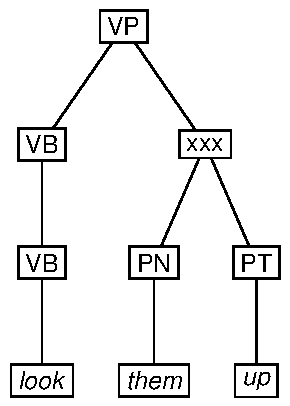
\includegraphics[width=0.3\textwidth,]{Images/graph9.jpg} \par\bgroup\index{tree=<tree>|exampleindex}\index{n=@n!<tree>|exampleindex}\index{arity=@arity!<tree>|exampleindex}\index{order=@order!<tree>|exampleindex}\index{ord=@ord!<tree>|exampleindex}\index{leaf=<leaf>|exampleindex}\index{parent=@parent!<leaf>|exampleindex}\index{label=<label>|exampleindex}\index{leaf=<leaf>|exampleindex}\index{parent=@parent!<leaf>|exampleindex}\index{label=<label>|exampleindex}\index{leaf=<leaf>|exampleindex}\index{parent=@parent!<leaf>|exampleindex}\index{label=<label>|exampleindex}\index{iNode=<iNode>|exampleindex}\index{parent=@parent!<iNode>|exampleindex}\index{children=@children!<iNode>|exampleindex}\index{label=<label>|exampleindex}\index{iNode=<iNode>|exampleindex}\index{parent=@parent!<iNode>|exampleindex}\index{children=@children!<iNode>|exampleindex}\index{label=<label>|exampleindex}\index{iNode=<iNode>|exampleindex}\index{parent=@parent!<iNode>|exampleindex}\index{children=@children!<iNode>|exampleindex}\index{follow=@follow!<iNode>|exampleindex}\index{label=<label>|exampleindex}\index{iNode=<iNode>|exampleindex}\index{parent=@parent!<iNode>|exampleindex}\index{children=@children!<iNode>|exampleindex}\index{label=<label>|exampleindex}\index{root=<root>|exampleindex}\index{children=@children!<root>|exampleindex}\index{label=<label>|exampleindex}\exampleFont \begin{shaded}\noindent\mbox{}{<\textbf{tree}\hspace*{1em}{n}="{ex4}"\hspace*{1em}{arity}="{2}"\hspace*{1em}{order}="{8}"\hspace*{1em}{ord}="{true}">}\mbox{}\newline 
\hspace*{1em}{<\textbf{leaf}\hspace*{1em}{xml:id}="{GD-LOOK1}"\hspace*{1em}{parent}="{\#GD-VB2}">}\mbox{}\newline 
\hspace*{1em}\hspace*{1em}{<\textbf{label}>}look{</\textbf{label}>}\mbox{}\newline 
\hspace*{1em}{</\textbf{leaf}>}\mbox{}\newline 
\hspace*{1em}{<\textbf{leaf}\hspace*{1em}{xml:id}="{GD-THEM1}"\hspace*{1em}{parent}="{\#GD-PN1}">}\mbox{}\newline 
\hspace*{1em}\hspace*{1em}{<\textbf{label}>}them{</\textbf{label}>}\mbox{}\newline 
\hspace*{1em}{</\textbf{leaf}>}\mbox{}\newline 
\hspace*{1em}{<\textbf{leaf}\hspace*{1em}{xml:id}="{GD-UP1}"\hspace*{1em}{parent}="{\#GD-PT1}">}\mbox{}\newline 
\hspace*{1em}\hspace*{1em}{<\textbf{label}>}up{</\textbf{label}>}\mbox{}\newline 
\hspace*{1em}{</\textbf{leaf}>}\mbox{}\newline 
\hspace*{1em}{<\textbf{iNode}\hspace*{1em}{xml:id}="{GD-VB2}"\hspace*{1em}{parent}="{\#GD-VB1}"\mbox{}\newline 
\hspace*{1em}\hspace*{1em}{children}="{\#GD-LOOK1}">}\mbox{}\newline 
\hspace*{1em}\hspace*{1em}{<\textbf{label}>}VB{</\textbf{label}>}\mbox{}\newline 
\hspace*{1em}{</\textbf{iNode}>}\mbox{}\newline 
\hspace*{1em}{<\textbf{iNode}\hspace*{1em}{xml:id}="{GD-PN1}"\hspace*{1em}{parent}="{\#GD-VP1}"\mbox{}\newline 
\hspace*{1em}\hspace*{1em}{children}="{\#GD-THEM1}">}\mbox{}\newline 
\hspace*{1em}\hspace*{1em}{<\textbf{label}>}PN{</\textbf{label}>}\mbox{}\newline 
\hspace*{1em}{</\textbf{iNode}>}\mbox{}\newline 
\hspace*{1em}{<\textbf{iNode}\hspace*{1em}{xml:id}="{GD-PT1}"\hspace*{1em}{parent}="{\#GD-VB1}"\mbox{}\newline 
\hspace*{1em}\hspace*{1em}{children}="{\#GD-UP1}"\hspace*{1em}{follow}="{\#GD-PN1}">}\mbox{}\newline 
\hspace*{1em}\hspace*{1em}{<\textbf{label}>}PT{</\textbf{label}>}\mbox{}\newline 
\hspace*{1em}{</\textbf{iNode}>}\mbox{}\newline 
\hspace*{1em}{<\textbf{iNode}\hspace*{1em}{xml:id}="{GD-VB1}"\hspace*{1em}{parent}="{\#GD-VP1}"\mbox{}\newline 
\hspace*{1em}\hspace*{1em}{children}="{\#GD-VB2 \#GD-PT1}">}\mbox{}\newline 
\hspace*{1em}\hspace*{1em}{<\textbf{label}>}VB{</\textbf{label}>}\mbox{}\newline 
\hspace*{1em}{</\textbf{iNode}>}\mbox{}\newline 
\hspace*{1em}{<\textbf{root}\hspace*{1em}{xml:id}="{GD-VP1}"\mbox{}\newline 
\hspace*{1em}\hspace*{1em}{children}="{\#GD-VB1 \#GD-PN1}">}\mbox{}\newline 
\hspace*{1em}\hspace*{1em}{<\textbf{label}>}VP{</\textbf{label}>}\mbox{}\newline 
\hspace*{1em}{</\textbf{root}>}\mbox{}\newline 
{</\textbf{tree}>}\end{shaded}\egroup\par 
\subsection[{Another Tree Notation}]{Another Tree Notation}\label{GDAT}\par
In this section, we present an alternative to the method of representing the structure of ordered rooted trees given in section \textit{\hyperref[GDTR]{19.2.\ Trees}}, which is based on the observation that any node of such a tree can be thought of as the root of the subtree that it dominates. Thus subtrees can be thought of as the same type as the trees they are embedded in, hence the designation \hyperref[TEI.eTree]{<eTree>}, for \textit{embedding tree}. Whereas in a \hyperref[TEI.tree]{<tree>} the relationship among the parts is indicated by the {\itshape children} attribute, and by the names of the elements \hyperref[TEI.root]{<root>}, \hyperref[TEI.iNode]{<iNode>}, and \hyperref[TEI.leaf]{<leaf>}, the relationship among the parts of an \hyperref[TEI.eTree]{<eTree>} is indicated simply by the arrangement of their content. However, we have chosen to enable encoders to distinguish the terminal elements of an \hyperref[TEI.eTree]{<eTree>} by means of the empty \hyperref[TEI.eLeaf]{<eLeaf>} element, though its use is not required; the \hyperref[TEI.eTree]{<eTree>} element can also be used to identify the terminal nodes of \hyperref[TEI.eTree]{<eTree>} elements. We also provide a \hyperref[TEI.triangle]{<triangle>} element, which can be thought of as an underspecified \hyperref[TEI.eTree]{<eTree>}, i.e. an \hyperref[TEI.eTree]{<eTree>} in which certain information has been left out. In addition, we provide a \hyperref[TEI.forest]{<forest>} element, which consists of one or more \hyperref[TEI.tree]{<tree>}, \hyperref[TEI.eTree]{<eTree>}, or \hyperref[TEI.triangle]{<triangle>} elements, and a \hyperref[TEI.listForest]{<listForest>} element, which consists of one or more \hyperref[TEI.forest]{<forest>} elements. The elements used for the encoding of embedding trees and the units containing them have the following descriptions and attributes. 
\begin{sansreflist}
  
\item [\textbf{<eTree>}] (embedding tree) provides an alternative to the \hyperref[TEI.tree]{<tree>} element for representing ordered rooted tree structures.\hfil\\[-10pt]\begin{sansreflist}
    \item[@{\itshape value}]
  provides the value of an embedding tree, which is a feature structure or other analytic element.
\end{sansreflist}  
\item [\textbf{<triangle>}] (underspecified embedding tree, so called because of its characteristic shape when drawn) provides for an underspecified \hyperref[TEI.eTree]{<eTree>}, that is, an \hyperref[TEI.eTree]{<eTree>} with information left out.\hfil\\[-10pt]\begin{sansreflist}
    \item[@{\itshape value}]
  supplies a value for the triangle, in the form of the identifier of a feature structure or other analytic element.
\end{sansreflist}  
\item [\textbf{<eLeaf>}] (leaf or terminal node of an embedding tree) provides explicitly for a leaf of an embedding tree, which may also be encoded with the \hyperref[TEI.eTree]{<eTree>} element.\hfil\\[-10pt]\begin{sansreflist}
    \item[@{\itshape value}]
  indicates the value of an embedding leaf, which is a feature structure or other analytic element.
\end{sansreflist}  
\item [\textbf{<forest>}] (forest) provides for groups of rooted trees.
\item [\textbf{<listForest>}] provides for lists of forests.
\end{sansreflist}
\par
Like the \hyperref[TEI.root]{<root>}, \hyperref[TEI.iNode]{<iNode>}, and \hyperref[TEI.leaf]{<leaf>} of a \hyperref[TEI.tree]{<tree>}, the \hyperref[TEI.eTree]{<eTree>}, \hyperref[TEI.triangle]{<triangle>} and \hyperref[TEI.eLeaf]{<eLeaf>} elements may also have {\itshape value} attributes and \hyperref[TEI.label]{<label>} children.\par
To illustrate the use of the \hyperref[TEI.eTree]{<eTree>} and \hyperref[TEI.eLeaf]{<eLeaf>} elements, here is an encoding of the second example in section \textit{\hyperref[GDTR]{19.2.\ Trees}}, repeated here for convenience.\par
 \noindent\includegraphics[width=0.3\textwidth,]{Images/graph10.jpg} \par\bgroup\index{eTree=<eTree>|exampleindex}\index{n=@n!<eTree>|exampleindex}\index{label=<label>|exampleindex}\index{eTree=<eTree>|exampleindex}\index{label=<label>|exampleindex}\index{eLeaf=<eLeaf>|exampleindex}\index{label=<label>|exampleindex}\index{eTree=<eTree>|exampleindex}\index{label=<label>|exampleindex}\index{eTree=<eTree>|exampleindex}\index{label=<label>|exampleindex}\index{eLeaf=<eLeaf>|exampleindex}\index{label=<label>|exampleindex}\index{eTree=<eTree>|exampleindex}\index{label=<label>|exampleindex}\index{eLeaf=<eLeaf>|exampleindex}\index{label=<label>|exampleindex}\exampleFont \begin{shaded}\noindent\mbox{}{<\textbf{eTree}\hspace*{1em}{n}="{ex1}">}\mbox{}\newline 
\hspace*{1em}{<\textbf{label}>}PP{</\textbf{label}>}\mbox{}\newline 
\hspace*{1em}{<\textbf{eTree}>}\mbox{}\newline 
\hspace*{1em}\hspace*{1em}{<\textbf{label}>}P{</\textbf{label}>}\mbox{}\newline 
\hspace*{1em}\hspace*{1em}{<\textbf{eLeaf}>}\mbox{}\newline 
\hspace*{1em}\hspace*{1em}\hspace*{1em}{<\textbf{label}>}with{</\textbf{label}>}\mbox{}\newline 
\hspace*{1em}\hspace*{1em}{</\textbf{eLeaf}>}\mbox{}\newline 
\hspace*{1em}{</\textbf{eTree}>}\mbox{}\newline 
\hspace*{1em}{<\textbf{eTree}>}\mbox{}\newline 
\hspace*{1em}\hspace*{1em}{<\textbf{label}>}NP{</\textbf{label}>}\mbox{}\newline 
\hspace*{1em}\hspace*{1em}{<\textbf{eTree}>}\mbox{}\newline 
\hspace*{1em}\hspace*{1em}\hspace*{1em}{<\textbf{label}>}Art{</\textbf{label}>}\mbox{}\newline 
\hspace*{1em}\hspace*{1em}\hspace*{1em}{<\textbf{eLeaf}>}\mbox{}\newline 
\hspace*{1em}\hspace*{1em}\hspace*{1em}\hspace*{1em}{<\textbf{label}>}the{</\textbf{label}>}\mbox{}\newline 
\hspace*{1em}\hspace*{1em}\hspace*{1em}{</\textbf{eLeaf}>}\mbox{}\newline 
\hspace*{1em}\hspace*{1em}{</\textbf{eTree}>}\mbox{}\newline 
\hspace*{1em}\hspace*{1em}{<\textbf{eTree}>}\mbox{}\newline 
\hspace*{1em}\hspace*{1em}\hspace*{1em}{<\textbf{label}>}N{</\textbf{label}>}\mbox{}\newline 
\hspace*{1em}\hspace*{1em}\hspace*{1em}{<\textbf{eLeaf}>}\mbox{}\newline 
\hspace*{1em}\hspace*{1em}\hspace*{1em}\hspace*{1em}{<\textbf{label}>}periscope{</\textbf{label}>}\mbox{}\newline 
\hspace*{1em}\hspace*{1em}\hspace*{1em}{</\textbf{eLeaf}>}\mbox{}\newline 
\hspace*{1em}\hspace*{1em}{</\textbf{eTree}>}\mbox{}\newline 
\hspace*{1em}{</\textbf{eTree}>}\mbox{}\newline 
{</\textbf{eTree}>}\end{shaded}\egroup\par \par
Next, we provide an encoding, using the \hyperref[TEI.triangle]{<triangle>} element, in which the internal structure of the \hyperref[TEI.eTree]{<eTree>} labeled \texttt{NP} is omitted.\par
 \noindent\includegraphics[width=0.3\textwidth,]{Images/graph11.jpg} \par\bgroup\index{eTree=<eTree>|exampleindex}\index{n=@n!<eTree>|exampleindex}\index{label=<label>|exampleindex}\index{eTree=<eTree>|exampleindex}\index{label=<label>|exampleindex}\index{eLeaf=<eLeaf>|exampleindex}\index{label=<label>|exampleindex}\index{triangle=<triangle>|exampleindex}\index{label=<label>|exampleindex}\index{eLeaf=<eLeaf>|exampleindex}\index{label=<label>|exampleindex}\exampleFont \begin{shaded}\noindent\mbox{}{<\textbf{eTree}\hspace*{1em}{n}="{ex2}">}\mbox{}\newline 
\hspace*{1em}{<\textbf{label}>}PP{</\textbf{label}>}\mbox{}\newline 
\hspace*{1em}{<\textbf{eTree}>}\mbox{}\newline 
\hspace*{1em}\hspace*{1em}{<\textbf{label}>}P{</\textbf{label}>}\mbox{}\newline 
\hspace*{1em}\hspace*{1em}{<\textbf{eLeaf}>}\mbox{}\newline 
\hspace*{1em}\hspace*{1em}\hspace*{1em}{<\textbf{label}>}with{</\textbf{label}>}\mbox{}\newline 
\hspace*{1em}\hspace*{1em}{</\textbf{eLeaf}>}\mbox{}\newline 
\hspace*{1em}{</\textbf{eTree}>}\mbox{}\newline 
\hspace*{1em}{<\textbf{triangle}>}\mbox{}\newline 
\hspace*{1em}\hspace*{1em}{<\textbf{label}>}NP{</\textbf{label}>}\mbox{}\newline 
\hspace*{1em}\hspace*{1em}{<\textbf{eLeaf}>}\mbox{}\newline 
\hspace*{1em}\hspace*{1em}\hspace*{1em}{<\textbf{label}>}the periscope{</\textbf{label}>}\mbox{}\newline 
\hspace*{1em}\hspace*{1em}{</\textbf{eLeaf}>}\mbox{}\newline 
\hspace*{1em}{</\textbf{triangle}>}\mbox{}\newline 
{</\textbf{eTree}>}\end{shaded}\egroup\par \par
Ambiguity involving alternative tree structures associated with the same terminal sequence can be encoded relatively conveniently using a combination of the {\itshape exclude} and {\itshape copyOf} attributes described in sections \textit{\hyperref[SAAT]{16.8.\ Alternation}} and \textit{\hyperref[SAIE]{16.6.\ Identical Elements and Virtual Copies}}. In the simplest case, an \hyperref[TEI.eTree]{<eTree>} may be part of the content of exactly one of two different \hyperref[TEI.eTree]{<eTree>} elements. To mark it up, the embedded \hyperref[TEI.eTree]{<eTree>} may be fully specified within one of the embedding \hyperref[TEI.eTree]{<eTree>} elements to which it may belong, and a virtual copy, specified by the {\itshape copyOf} attribute, may appear on the other. In addition, each of the embedded elements in question is specified as excluding the other, using the {\itshape exclude} attribute. To illustrate, consider the English phrase \textit{see the vessel with the periscope}, which may be considered to be structurally ambiguous, depending on whether the phrase \textit{with the periscope} is a modifier of the phrase \textit{the vessel} or a modifier of the phrase \textit{see the vessel}. This ambiguity is indicated in the sketch of the ambiguous tree by means of the dotted-line arcs. The markup using the {\itshape copyOf} and {\itshape exclude} attributes follows the sketch.\par
 \noindent\includegraphics[width=0.8\textwidth,]{Images/graph12.jpg} \par\bgroup\index{eTree=<eTree>|exampleindex}\index{n=@n!<eTree>|exampleindex}\index{label=<label>|exampleindex}\index{eTree=<eTree>|exampleindex}\index{label=<label>|exampleindex}\index{eLeaf=<eLeaf>|exampleindex}\index{label=<label>|exampleindex}\index{eTree=<eTree>|exampleindex}\index{label=<label>|exampleindex}\index{eTree=<eTree>|exampleindex}\index{label=<label>|exampleindex}\index{eLeaf=<eLeaf>|exampleindex}\index{label=<label>|exampleindex}\index{eTree=<eTree>|exampleindex}\index{label=<label>|exampleindex}\index{eLeaf=<eLeaf>|exampleindex}\index{label=<label>|exampleindex}\index{eTree=<eTree>|exampleindex}\index{exclude=@exclude!<eTree>|exampleindex}\index{label=<label>|exampleindex}\index{eTree=<eTree>|exampleindex}\index{label=<label>|exampleindex}\index{eLeaf=<eLeaf>|exampleindex}\index{label=<label>|exampleindex}\index{eTree=<eTree>|exampleindex}\index{label=<label>|exampleindex}\index{eTree=<eTree>|exampleindex}\index{label=<label>|exampleindex}\index{eLeaf=<eLeaf>|exampleindex}\index{label=<label>|exampleindex}\index{eTree=<eTree>|exampleindex}\index{label=<label>|exampleindex}\index{eLeaf=<eLeaf>|exampleindex}\index{label=<label>|exampleindex}\index{eTree=<eTree>|exampleindex}\index{copyOf=@copyOf!<eTree>|exampleindex}\index{exclude=@exclude!<eTree>|exampleindex}\index{label=<label>|exampleindex}\exampleFont \begin{shaded}\noindent\mbox{}{<\textbf{eTree}\hspace*{1em}{n}="{ex3}">}\mbox{}\newline 
\hspace*{1em}{<\textbf{label}>}VP{</\textbf{label}>}\mbox{}\newline 
\hspace*{1em}{<\textbf{eTree}>}\mbox{}\newline 
\hspace*{1em}\hspace*{1em}{<\textbf{label}>}V{</\textbf{label}>}\mbox{}\newline 
\hspace*{1em}\hspace*{1em}{<\textbf{eLeaf}>}\mbox{}\newline 
\hspace*{1em}\hspace*{1em}\hspace*{1em}{<\textbf{label}>}see{</\textbf{label}>}\mbox{}\newline 
\hspace*{1em}\hspace*{1em}{</\textbf{eLeaf}>}\mbox{}\newline 
\hspace*{1em}{</\textbf{eTree}>}\mbox{}\newline 
\hspace*{1em}{<\textbf{eTree}>}\mbox{}\newline 
\hspace*{1em}\hspace*{1em}{<\textbf{label}>}NP{</\textbf{label}>}\mbox{}\newline 
\hspace*{1em}\hspace*{1em}{<\textbf{eTree}>}\mbox{}\newline 
\hspace*{1em}\hspace*{1em}\hspace*{1em}{<\textbf{label}>}Art{</\textbf{label}>}\mbox{}\newline 
\hspace*{1em}\hspace*{1em}\hspace*{1em}{<\textbf{eLeaf}>}\mbox{}\newline 
\hspace*{1em}\hspace*{1em}\hspace*{1em}\hspace*{1em}{<\textbf{label}>}the{</\textbf{label}>}\mbox{}\newline 
\hspace*{1em}\hspace*{1em}\hspace*{1em}{</\textbf{eLeaf}>}\mbox{}\newline 
\hspace*{1em}\hspace*{1em}{</\textbf{eTree}>}\mbox{}\newline 
\hspace*{1em}\hspace*{1em}{<\textbf{eTree}>}\mbox{}\newline 
\hspace*{1em}\hspace*{1em}\hspace*{1em}{<\textbf{label}>}N{</\textbf{label}>}\mbox{}\newline 
\hspace*{1em}\hspace*{1em}\hspace*{1em}{<\textbf{eLeaf}>}\mbox{}\newline 
\hspace*{1em}\hspace*{1em}\hspace*{1em}\hspace*{1em}{<\textbf{label}>}vessel{</\textbf{label}>}\mbox{}\newline 
\hspace*{1em}\hspace*{1em}\hspace*{1em}{</\textbf{eLeaf}>}\mbox{}\newline 
\hspace*{1em}\hspace*{1em}{</\textbf{eTree}>}\mbox{}\newline 
\hspace*{1em}\hspace*{1em}{<\textbf{eTree}\hspace*{1em}{xml:id}="{GD-PPA}"\hspace*{1em}{exclude}="{\#GD-PPB}">}\mbox{}\newline 
\hspace*{1em}\hspace*{1em}\hspace*{1em}{<\textbf{label}>}PP{</\textbf{label}>}\mbox{}\newline 
\hspace*{1em}\hspace*{1em}\hspace*{1em}{<\textbf{eTree}>}\mbox{}\newline 
\hspace*{1em}\hspace*{1em}\hspace*{1em}\hspace*{1em}{<\textbf{label}>}P{</\textbf{label}>}\mbox{}\newline 
\hspace*{1em}\hspace*{1em}\hspace*{1em}\hspace*{1em}{<\textbf{eLeaf}>}\mbox{}\newline 
\hspace*{1em}\hspace*{1em}\hspace*{1em}\hspace*{1em}\hspace*{1em}{<\textbf{label}>}with{</\textbf{label}>}\mbox{}\newline 
\hspace*{1em}\hspace*{1em}\hspace*{1em}\hspace*{1em}{</\textbf{eLeaf}>}\mbox{}\newline 
\hspace*{1em}\hspace*{1em}\hspace*{1em}{</\textbf{eTree}>}\mbox{}\newline 
\hspace*{1em}\hspace*{1em}\hspace*{1em}{<\textbf{eTree}>}\mbox{}\newline 
\hspace*{1em}\hspace*{1em}\hspace*{1em}\hspace*{1em}{<\textbf{label}>}NP{</\textbf{label}>}\mbox{}\newline 
\hspace*{1em}\hspace*{1em}\hspace*{1em}\hspace*{1em}{<\textbf{eTree}>}\mbox{}\newline 
\hspace*{1em}\hspace*{1em}\hspace*{1em}\hspace*{1em}\hspace*{1em}{<\textbf{label}>}Art{</\textbf{label}>}\mbox{}\newline 
\hspace*{1em}\hspace*{1em}\hspace*{1em}\hspace*{1em}\hspace*{1em}{<\textbf{eLeaf}>}\mbox{}\newline 
\hspace*{1em}\hspace*{1em}\hspace*{1em}\hspace*{1em}\hspace*{1em}\hspace*{1em}{<\textbf{label}>}the{</\textbf{label}>}\mbox{}\newline 
\hspace*{1em}\hspace*{1em}\hspace*{1em}\hspace*{1em}\hspace*{1em}{</\textbf{eLeaf}>}\mbox{}\newline 
\hspace*{1em}\hspace*{1em}\hspace*{1em}\hspace*{1em}{</\textbf{eTree}>}\mbox{}\newline 
\hspace*{1em}\hspace*{1em}\hspace*{1em}\hspace*{1em}{<\textbf{eTree}>}\mbox{}\newline 
\hspace*{1em}\hspace*{1em}\hspace*{1em}\hspace*{1em}\hspace*{1em}{<\textbf{label}>}N{</\textbf{label}>}\mbox{}\newline 
\hspace*{1em}\hspace*{1em}\hspace*{1em}\hspace*{1em}\hspace*{1em}{<\textbf{eLeaf}>}\mbox{}\newline 
\hspace*{1em}\hspace*{1em}\hspace*{1em}\hspace*{1em}\hspace*{1em}\hspace*{1em}{<\textbf{label}>}periscope{</\textbf{label}>}\mbox{}\newline 
\hspace*{1em}\hspace*{1em}\hspace*{1em}\hspace*{1em}\hspace*{1em}{</\textbf{eLeaf}>}\mbox{}\newline 
\hspace*{1em}\hspace*{1em}\hspace*{1em}\hspace*{1em}{</\textbf{eTree}>}\mbox{}\newline 
\hspace*{1em}\hspace*{1em}\hspace*{1em}{</\textbf{eTree}>}\mbox{}\newline 
\hspace*{1em}\hspace*{1em}{</\textbf{eTree}>}\mbox{}\newline 
\hspace*{1em}{</\textbf{eTree}>}\mbox{}\newline 
\hspace*{1em}{<\textbf{eTree}\hspace*{1em}{xml:id}="{GD-PPB}"\hspace*{1em}{copyOf}="{\#GD-PPA}"\mbox{}\newline 
\hspace*{1em}\hspace*{1em}{exclude}="{\#GD-PPA}">}\mbox{}\newline 
\hspace*{1em}\hspace*{1em}{<\textbf{label}>}PP{</\textbf{label}>}\mbox{}\newline 
\hspace*{1em}{</\textbf{eTree}>}\mbox{}\newline 
{</\textbf{eTree}>}\end{shaded}\egroup\par \par
To indicate that one of the alternatives is selected, one may specify the {\itshape select} attribute on the highest \hyperref[TEI.eTree]{<eTree>} as either \#GD-PPA or \#GD-PPB; see section \textit{\hyperref[SAAT]{16.8.\ Alternation}}.\par
Depending on the grammar one uses to associate structures with examples like \textit{see the man with the periscope}, the representations may be more complicated than this. For example, adopting a version of the \textit{X-bar} theory of phrase structure originated by Jackendoff,\footnote{\cite{GD-BIBL-2}} the attachment of a modifier may require the creation of an intermediate node which is not required when the attachment is not made, as shown in the following diagram. A possible encoding of this ambiguous structure immediately follows the diagram.\par
 \noindent\includegraphics[width=0.8\textwidth,]{Images/graph13.jpg} \par\bgroup\index{eTree=<eTree>|exampleindex}\index{n=@n!<eTree>|exampleindex}\index{label=<label>|exampleindex}\index{eTree=<eTree>|exampleindex}\index{exclude=@exclude!<eTree>|exampleindex}\index{label=<label>|exampleindex}\index{eTree=<eTree>|exampleindex}\index{label=<label>|exampleindex}\index{eLeaf=<eLeaf>|exampleindex}\index{label=<label>|exampleindex}\index{eTree=<eTree>|exampleindex}\index{label=<label>|exampleindex}\index{eTree=<eTree>|exampleindex}\index{label=<label>|exampleindex}\index{eLeaf=<eLeaf>|exampleindex}\index{label=<label>|exampleindex}\index{eTree=<eTree>|exampleindex}\index{label=<label>|exampleindex}\index{eTree=<eTree>|exampleindex}\index{label=<label>|exampleindex}\index{eTree=<eTree>|exampleindex}\index{label=<label>|exampleindex}\index{eLeaf=<eLeaf>|exampleindex}\index{label=<label>|exampleindex}\index{eTree=<eTree>|exampleindex}\index{label=<label>|exampleindex}\index{eTree=<eTree>|exampleindex}\index{label=<label>|exampleindex}\index{eLeaf=<eLeaf>|exampleindex}\index{label=<label>|exampleindex}\index{eTree=<eTree>|exampleindex}\index{label=<label>|exampleindex}\index{eTree=<eTree>|exampleindex}\index{label=<label>|exampleindex}\index{eLeaf=<eLeaf>|exampleindex}\index{label=<label>|exampleindex}\index{eTree=<eTree>|exampleindex}\index{label=<label>|exampleindex}\index{eTree=<eTree>|exampleindex}\index{label=<label>|exampleindex}\index{eLeaf=<eLeaf>|exampleindex}\index{label=<label>|exampleindex}\index{eTree=<eTree>|exampleindex}\index{exclude=@exclude!<eTree>|exampleindex}\index{label=<label>|exampleindex}\index{eTree=<eTree>|exampleindex}\index{label=<label>|exampleindex}\index{eTree=<eTree>|exampleindex}\index{copyOf=@copyOf!<eTree>|exampleindex}\index{label=<label>|exampleindex}\index{eTree=<eTree>|exampleindex}\index{label=<label>|exampleindex}\index{eTree=<eTree>|exampleindex}\index{copyOf=@copyOf!<eTree>|exampleindex}\index{label=<label>|exampleindex}\index{eTree=<eTree>|exampleindex}\index{copyOf=@copyOf!<eTree>|exampleindex}\index{label=<label>|exampleindex}\index{eTree=<eTree>|exampleindex}\index{copyOf=@copyOf!<eTree>|exampleindex}\index{label=<label>|exampleindex}\exampleFont \begin{shaded}\noindent\mbox{}{<\textbf{eTree}\hspace*{1em}{n}="{ex4}">}\mbox{}\newline 
\hspace*{1em}{<\textbf{label}>}VP{</\textbf{label}>}\mbox{}\newline 
\hspace*{1em}{<\textbf{eTree}\hspace*{1em}{xml:id}="{VBARA}"\hspace*{1em}{exclude}="{\#VBARB}">}\mbox{}\newline 
\hspace*{1em}\hspace*{1em}{<\textbf{label}>}V'{</\textbf{label}>}\mbox{}\newline 
\hspace*{1em}\hspace*{1em}{<\textbf{eTree}\hspace*{1em}{xml:id}="{VA}">}\mbox{}\newline 
\hspace*{1em}\hspace*{1em}\hspace*{1em}{<\textbf{label}>}V{</\textbf{label}>}\mbox{}\newline 
\hspace*{1em}\hspace*{1em}\hspace*{1em}{<\textbf{eLeaf}>}\mbox{}\newline 
\hspace*{1em}\hspace*{1em}\hspace*{1em}\hspace*{1em}{<\textbf{label}>}see{</\textbf{label}>}\mbox{}\newline 
\hspace*{1em}\hspace*{1em}\hspace*{1em}{</\textbf{eLeaf}>}\mbox{}\newline 
\hspace*{1em}\hspace*{1em}{</\textbf{eTree}>}\mbox{}\newline 
\hspace*{1em}\hspace*{1em}{<\textbf{eTree}>}\mbox{}\newline 
\hspace*{1em}\hspace*{1em}\hspace*{1em}{<\textbf{label}>}NP{</\textbf{label}>}\mbox{}\newline 
\hspace*{1em}\hspace*{1em}\hspace*{1em}{<\textbf{eTree}\hspace*{1em}{xml:id}="{SPEC1A}">}\mbox{}\newline 
\hspace*{1em}\hspace*{1em}\hspace*{1em}\hspace*{1em}{<\textbf{label}>}Spec{</\textbf{label}>}\mbox{}\newline 
\hspace*{1em}\hspace*{1em}\hspace*{1em}\hspace*{1em}{<\textbf{eLeaf}>}\mbox{}\newline 
\hspace*{1em}\hspace*{1em}\hspace*{1em}\hspace*{1em}\hspace*{1em}{<\textbf{label}>}the{</\textbf{label}>}\mbox{}\newline 
\hspace*{1em}\hspace*{1em}\hspace*{1em}\hspace*{1em}{</\textbf{eLeaf}>}\mbox{}\newline 
\hspace*{1em}\hspace*{1em}\hspace*{1em}{</\textbf{eTree}>}\mbox{}\newline 
\hspace*{1em}\hspace*{1em}\hspace*{1em}{<\textbf{eTree}>}\mbox{}\newline 
\hspace*{1em}\hspace*{1em}\hspace*{1em}\hspace*{1em}{<\textbf{label}>}N'{</\textbf{label}>}\mbox{}\newline 
\hspace*{1em}\hspace*{1em}\hspace*{1em}\hspace*{1em}{<\textbf{eTree}\hspace*{1em}{xml:id}="{NBAR2A}">}\mbox{}\newline 
\hspace*{1em}\hspace*{1em}\hspace*{1em}\hspace*{1em}\hspace*{1em}{<\textbf{label}>}N'{</\textbf{label}>}\mbox{}\newline 
\hspace*{1em}\hspace*{1em}\hspace*{1em}\hspace*{1em}\hspace*{1em}{<\textbf{eTree}>}\mbox{}\newline 
\hspace*{1em}\hspace*{1em}\hspace*{1em}\hspace*{1em}\hspace*{1em}\hspace*{1em}{<\textbf{label}>}N{</\textbf{label}>}\mbox{}\newline 
\hspace*{1em}\hspace*{1em}\hspace*{1em}\hspace*{1em}\hspace*{1em}\hspace*{1em}{<\textbf{eLeaf}>}\mbox{}\newline 
\hspace*{1em}\hspace*{1em}\hspace*{1em}\hspace*{1em}\hspace*{1em}\hspace*{1em}\hspace*{1em}{<\textbf{label}>}vessel{</\textbf{label}>}\mbox{}\newline 
\hspace*{1em}\hspace*{1em}\hspace*{1em}\hspace*{1em}\hspace*{1em}\hspace*{1em}{</\textbf{eLeaf}>}\mbox{}\newline 
\hspace*{1em}\hspace*{1em}\hspace*{1em}\hspace*{1em}\hspace*{1em}{</\textbf{eTree}>}\mbox{}\newline 
\hspace*{1em}\hspace*{1em}\hspace*{1em}\hspace*{1em}{</\textbf{eTree}>}\mbox{}\newline 
\hspace*{1em}\hspace*{1em}\hspace*{1em}\hspace*{1em}{<\textbf{eTree}\hspace*{1em}{xml:id}="{PPA1}">}\mbox{}\newline 
\hspace*{1em}\hspace*{1em}\hspace*{1em}\hspace*{1em}\hspace*{1em}{<\textbf{label}>}PP{</\textbf{label}>}\mbox{}\newline 
\hspace*{1em}\hspace*{1em}\hspace*{1em}\hspace*{1em}\hspace*{1em}{<\textbf{eTree}>}\mbox{}\newline 
\hspace*{1em}\hspace*{1em}\hspace*{1em}\hspace*{1em}\hspace*{1em}\hspace*{1em}{<\textbf{label}>}P{</\textbf{label}>}\mbox{}\newline 
\hspace*{1em}\hspace*{1em}\hspace*{1em}\hspace*{1em}\hspace*{1em}\hspace*{1em}{<\textbf{eLeaf}>}\mbox{}\newline 
\hspace*{1em}\hspace*{1em}\hspace*{1em}\hspace*{1em}\hspace*{1em}\hspace*{1em}\hspace*{1em}{<\textbf{label}>}with{</\textbf{label}>}\mbox{}\newline 
\hspace*{1em}\hspace*{1em}\hspace*{1em}\hspace*{1em}\hspace*{1em}\hspace*{1em}{</\textbf{eLeaf}>}\mbox{}\newline 
\hspace*{1em}\hspace*{1em}\hspace*{1em}\hspace*{1em}\hspace*{1em}{</\textbf{eTree}>}\mbox{}\newline 
\hspace*{1em}\hspace*{1em}\hspace*{1em}\hspace*{1em}\hspace*{1em}{<\textbf{eTree}>}\mbox{}\newline 
\hspace*{1em}\hspace*{1em}\hspace*{1em}\hspace*{1em}\hspace*{1em}\hspace*{1em}{<\textbf{label}>}NP{</\textbf{label}>}\mbox{}\newline 
\hspace*{1em}\hspace*{1em}\hspace*{1em}\hspace*{1em}\hspace*{1em}\hspace*{1em}{<\textbf{eTree}>}\mbox{}\newline 
\hspace*{1em}\hspace*{1em}\hspace*{1em}\hspace*{1em}\hspace*{1em}\hspace*{1em}\hspace*{1em}{<\textbf{label}>}Spec{</\textbf{label}>}\mbox{}\newline 
\hspace*{1em}\hspace*{1em}\hspace*{1em}\hspace*{1em}\hspace*{1em}\hspace*{1em}\hspace*{1em}{<\textbf{eLeaf}>}\mbox{}\newline 
\hspace*{1em}\hspace*{1em}\hspace*{1em}\hspace*{1em}\hspace*{1em}\hspace*{1em}\hspace*{1em}\hspace*{1em}{<\textbf{label}>}the{</\textbf{label}>}\mbox{}\newline 
\hspace*{1em}\hspace*{1em}\hspace*{1em}\hspace*{1em}\hspace*{1em}\hspace*{1em}\hspace*{1em}{</\textbf{eLeaf}>}\mbox{}\newline 
\hspace*{1em}\hspace*{1em}\hspace*{1em}\hspace*{1em}\hspace*{1em}\hspace*{1em}{</\textbf{eTree}>}\mbox{}\newline 
\hspace*{1em}\hspace*{1em}\hspace*{1em}\hspace*{1em}\hspace*{1em}\hspace*{1em}{<\textbf{eTree}>}\mbox{}\newline 
\hspace*{1em}\hspace*{1em}\hspace*{1em}\hspace*{1em}\hspace*{1em}\hspace*{1em}\hspace*{1em}{<\textbf{label}>}N'{</\textbf{label}>}\mbox{}\newline 
\hspace*{1em}\hspace*{1em}\hspace*{1em}\hspace*{1em}\hspace*{1em}\hspace*{1em}\hspace*{1em}{<\textbf{eTree}>}\mbox{}\newline 
\hspace*{1em}\hspace*{1em}\hspace*{1em}\hspace*{1em}\hspace*{1em}\hspace*{1em}\hspace*{1em}\hspace*{1em}{<\textbf{label}>}N{</\textbf{label}>}\mbox{}\newline 
\hspace*{1em}\hspace*{1em}\hspace*{1em}\hspace*{1em}\hspace*{1em}\hspace*{1em}\hspace*{1em}\hspace*{1em}{<\textbf{eLeaf}>}\mbox{}\newline 
\hspace*{1em}\hspace*{1em}\hspace*{1em}\hspace*{1em}\hspace*{1em}\hspace*{1em}\hspace*{1em}\hspace*{1em}\hspace*{1em}{<\textbf{label}>}periscope{</\textbf{label}>}\mbox{}\newline 
\hspace*{1em}\hspace*{1em}\hspace*{1em}\hspace*{1em}\hspace*{1em}\hspace*{1em}\hspace*{1em}\hspace*{1em}{</\textbf{eLeaf}>}\mbox{}\newline 
\hspace*{1em}\hspace*{1em}\hspace*{1em}\hspace*{1em}\hspace*{1em}\hspace*{1em}\hspace*{1em}{</\textbf{eTree}>}\mbox{}\newline 
\hspace*{1em}\hspace*{1em}\hspace*{1em}\hspace*{1em}\hspace*{1em}\hspace*{1em}{</\textbf{eTree}>}\mbox{}\newline 
\hspace*{1em}\hspace*{1em}\hspace*{1em}\hspace*{1em}\hspace*{1em}{</\textbf{eTree}>}\mbox{}\newline 
\hspace*{1em}\hspace*{1em}\hspace*{1em}\hspace*{1em}{</\textbf{eTree}>}\mbox{}\newline 
\hspace*{1em}\hspace*{1em}\hspace*{1em}{</\textbf{eTree}>}\mbox{}\newline 
\hspace*{1em}\hspace*{1em}{</\textbf{eTree}>}\mbox{}\newline 
\hspace*{1em}{</\textbf{eTree}>}\mbox{}\newline 
\hspace*{1em}{<\textbf{eTree}\hspace*{1em}{xml:id}="{VBARB}"\hspace*{1em}{exclude}="{\#VBARA}">}\mbox{}\newline 
\hspace*{1em}\hspace*{1em}{<\textbf{label}>}V'{</\textbf{label}>}\mbox{}\newline 
\hspace*{1em}\hspace*{1em}{<\textbf{eTree}>}\mbox{}\newline 
\hspace*{1em}\hspace*{1em}\hspace*{1em}{<\textbf{label}>}V'{</\textbf{label}>}\mbox{}\newline 
\hspace*{1em}\hspace*{1em}\hspace*{1em}{<\textbf{eTree}\hspace*{1em}{xml:id}="{VB}"\hspace*{1em}{copyOf}="{\#VA}">}\mbox{}\newline 
\hspace*{1em}\hspace*{1em}\hspace*{1em}\hspace*{1em}{<\textbf{label}>}V{</\textbf{label}>}\mbox{}\newline 
\hspace*{1em}\hspace*{1em}\hspace*{1em}{</\textbf{eTree}>}\mbox{}\newline 
\hspace*{1em}\hspace*{1em}\hspace*{1em}{<\textbf{eTree}>}\mbox{}\newline 
\hspace*{1em}\hspace*{1em}\hspace*{1em}\hspace*{1em}{<\textbf{label}>}NP{</\textbf{label}>}\mbox{}\newline 
\hspace*{1em}\hspace*{1em}\hspace*{1em}\hspace*{1em}{<\textbf{eTree}\hspace*{1em}{xml:id}="{SPEC1B}"\hspace*{1em}{copyOf}="{\#SPEC1A}">}\mbox{}\newline 
\hspace*{1em}\hspace*{1em}\hspace*{1em}\hspace*{1em}\hspace*{1em}{<\textbf{label}>}Spec{</\textbf{label}>}\mbox{}\newline 
\hspace*{1em}\hspace*{1em}\hspace*{1em}\hspace*{1em}{</\textbf{eTree}>}\mbox{}\newline 
\hspace*{1em}\hspace*{1em}\hspace*{1em}\hspace*{1em}{<\textbf{eTree}\hspace*{1em}{xml:id}="{NBAR2B}"\hspace*{1em}{copyOf}="{\#NBAR2A}">}\mbox{}\newline 
\hspace*{1em}\hspace*{1em}\hspace*{1em}\hspace*{1em}\hspace*{1em}{<\textbf{label}>}N'{</\textbf{label}>}\mbox{}\newline 
\hspace*{1em}\hspace*{1em}\hspace*{1em}\hspace*{1em}{</\textbf{eTree}>}\mbox{}\newline 
\hspace*{1em}\hspace*{1em}\hspace*{1em}{</\textbf{eTree}>}\mbox{}\newline 
\hspace*{1em}\hspace*{1em}{</\textbf{eTree}>}\mbox{}\newline 
\hspace*{1em}\hspace*{1em}{<\textbf{eTree}\hspace*{1em}{xml:id}="{PPB}"\hspace*{1em}{copyOf}="{\#PPA1}">}\mbox{}\newline 
\hspace*{1em}\hspace*{1em}\hspace*{1em}{<\textbf{label}>}PP{</\textbf{label}>}\mbox{}\newline 
\hspace*{1em}\hspace*{1em}{</\textbf{eTree}>}\mbox{}\newline 
\hspace*{1em}{</\textbf{eTree}>}\mbox{}\newline 
{</\textbf{eTree}>}\end{shaded}\egroup\par \par
A \textit{derivation} in a generative grammar is often thought of as a set of trees. To encode such a derivation, one may use the \hyperref[TEI.forest]{<forest>} element, in which the trees may be marked up using the \hyperref[TEI.tree]{<tree>}, the \hyperref[TEI.eTree]{<eTree>}, or the \hyperref[TEI.triangle]{<triangle>} element. The {\itshape type} attribute may be used to specify what kind of derivation it is. Here is an example of a two-tree forest, involving application of the ‘wh-movement’ transformation in the derivation of \textit{what you do} (as in \textit{this is what you do}) from the underlying \textit{you do what}.\footnote{The symbols \texttt{e} and \texttt{t} denote special theoretical constructs (\textit{empty category} and \textit{trace} respectively), which need not concern us here.}\par
 \noindent\includegraphics[width=0.8\textwidth,]{Images/graph14.jpg} \par\bgroup\index{forest=<forest>|exampleindex}\index{n=@n!<forest>|exampleindex}\index{type=@type!<forest>|exampleindex}\index{eTree=<eTree>|exampleindex}\index{n=@n!<eTree>|exampleindex}\index{label=<label>|exampleindex}\index{eTree=<eTree>|exampleindex}\index{label=<label>|exampleindex}\index{eLeaf=<eLeaf>|exampleindex}\index{label=<label>|exampleindex}\index{eTree=<eTree>|exampleindex}\index{label=<label>|exampleindex}\index{eTree=<eTree>|exampleindex}\index{label=<label>|exampleindex}\index{eLeaf=<eLeaf>|exampleindex}\index{label=<label>|exampleindex}\index{eTree=<eTree>|exampleindex}\index{label=<label>|exampleindex}\index{eTree=<eTree>|exampleindex}\index{label=<label>|exampleindex}\index{eLeaf=<eLeaf>|exampleindex}\index{label=<label>|exampleindex}\index{eTree=<eTree>|exampleindex}\index{label=<label>|exampleindex}\index{eLeaf=<eLeaf>|exampleindex}\index{label=<label>|exampleindex}\index{eTree=<eTree>|exampleindex}\index{n=@n!<eTree>|exampleindex}\index{corresp=@corresp!<eTree>|exampleindex}\index{label=<label>|exampleindex}\index{eTree=<eTree>|exampleindex}\index{corresp=@corresp!<eTree>|exampleindex}\index{label=<label>|exampleindex}\index{eTree=<eTree>|exampleindex}\index{copyOf=@copyOf!<eTree>|exampleindex}\index{corresp=@corresp!<eTree>|exampleindex}\index{label=<label>|exampleindex}\index{eTree=<eTree>|exampleindex}\index{corresp=@corresp!<eTree>|exampleindex}\index{label=<label>|exampleindex}\index{eTree=<eTree>|exampleindex}\index{copyOf=@copyOf!<eTree>|exampleindex}\index{label=<label>|exampleindex}\index{eTree=<eTree>|exampleindex}\index{corresp=@corresp!<eTree>|exampleindex}\index{label=<label>|exampleindex}\index{eTree=<eTree>|exampleindex}\index{copyOf=@copyOf!<eTree>|exampleindex}\index{label=<label>|exampleindex}\index{eTree=<eTree>|exampleindex}\index{corresp=@corresp!<eTree>|exampleindex}\index{label=<label>|exampleindex}\index{eLeaf=<eLeaf>|exampleindex}\index{corresp=@corresp!<eLeaf>|exampleindex}\index{label=<label>|exampleindex}\exampleFont \begin{shaded}\noindent\mbox{}{<\textbf{forest}\hspace*{1em}{n}="{ex5}"\hspace*{1em}{type}="{derivation-syntactic}">}\mbox{}\newline 
\hspace*{1em}{<\textbf{eTree}\hspace*{1em}{n}="{Stage 1}"\hspace*{1em}{xml:id}="{S1SBAR}">}\mbox{}\newline 
\hspace*{1em}\hspace*{1em}{<\textbf{label}>}S'{</\textbf{label}>}\mbox{}\newline 
\hspace*{1em}\hspace*{1em}{<\textbf{eTree}\hspace*{1em}{xml:id}="{S1COMP}">}\mbox{}\newline 
\hspace*{1em}\hspace*{1em}\hspace*{1em}{<\textbf{label}>}COMP{</\textbf{label}>}\mbox{}\newline 
\hspace*{1em}\hspace*{1em}\hspace*{1em}{<\textbf{eLeaf}\hspace*{1em}{xml:id}="{S1E}">}\mbox{}\newline 
\hspace*{1em}\hspace*{1em}\hspace*{1em}\hspace*{1em}{<\textbf{label}>}e{</\textbf{label}>}\mbox{}\newline 
\hspace*{1em}\hspace*{1em}\hspace*{1em}{</\textbf{eLeaf}>}\mbox{}\newline 
\hspace*{1em}\hspace*{1em}{</\textbf{eTree}>}\mbox{}\newline 
\hspace*{1em}\hspace*{1em}{<\textbf{eTree}\hspace*{1em}{xml:id}="{S1S}">}\mbox{}\newline 
\hspace*{1em}\hspace*{1em}\hspace*{1em}{<\textbf{label}>}S{</\textbf{label}>}\mbox{}\newline 
\hspace*{1em}\hspace*{1em}\hspace*{1em}{<\textbf{eTree}\hspace*{1em}{xml:id}="{S1NP1}">}\mbox{}\newline 
\hspace*{1em}\hspace*{1em}\hspace*{1em}\hspace*{1em}{<\textbf{label}>}NP{</\textbf{label}>}\mbox{}\newline 
\hspace*{1em}\hspace*{1em}\hspace*{1em}\hspace*{1em}{<\textbf{eLeaf}>}\mbox{}\newline 
\hspace*{1em}\hspace*{1em}\hspace*{1em}\hspace*{1em}\hspace*{1em}{<\textbf{label}>}you{</\textbf{label}>}\mbox{}\newline 
\hspace*{1em}\hspace*{1em}\hspace*{1em}\hspace*{1em}{</\textbf{eLeaf}>}\mbox{}\newline 
\hspace*{1em}\hspace*{1em}\hspace*{1em}{</\textbf{eTree}>}\mbox{}\newline 
\hspace*{1em}\hspace*{1em}\hspace*{1em}{<\textbf{eTree}\hspace*{1em}{xml:id}="{S1VP}">}\mbox{}\newline 
\hspace*{1em}\hspace*{1em}\hspace*{1em}\hspace*{1em}{<\textbf{label}>}VP{</\textbf{label}>}\mbox{}\newline 
\hspace*{1em}\hspace*{1em}\hspace*{1em}\hspace*{1em}{<\textbf{eTree}\hspace*{1em}{xml:id}="{S1V}">}\mbox{}\newline 
\hspace*{1em}\hspace*{1em}\hspace*{1em}\hspace*{1em}\hspace*{1em}{<\textbf{label}>}V{</\textbf{label}>}\mbox{}\newline 
\hspace*{1em}\hspace*{1em}\hspace*{1em}\hspace*{1em}\hspace*{1em}{<\textbf{eLeaf}>}\mbox{}\newline 
\hspace*{1em}\hspace*{1em}\hspace*{1em}\hspace*{1em}\hspace*{1em}\hspace*{1em}{<\textbf{label}>}do{</\textbf{label}>}\mbox{}\newline 
\hspace*{1em}\hspace*{1em}\hspace*{1em}\hspace*{1em}\hspace*{1em}{</\textbf{eLeaf}>}\mbox{}\newline 
\hspace*{1em}\hspace*{1em}\hspace*{1em}\hspace*{1em}{</\textbf{eTree}>}\mbox{}\newline 
\hspace*{1em}\hspace*{1em}\hspace*{1em}\hspace*{1em}{<\textbf{eTree}\hspace*{1em}{xml:id}="{S1NP2}">}\mbox{}\newline 
\hspace*{1em}\hspace*{1em}\hspace*{1em}\hspace*{1em}\hspace*{1em}{<\textbf{label}>}NP{</\textbf{label}>}\mbox{}\newline 
\hspace*{1em}\hspace*{1em}\hspace*{1em}\hspace*{1em}\hspace*{1em}{<\textbf{eLeaf}\hspace*{1em}{xml:id}="{S1WH}">}\mbox{}\newline 
\hspace*{1em}\hspace*{1em}\hspace*{1em}\hspace*{1em}\hspace*{1em}\hspace*{1em}{<\textbf{label}>}what{</\textbf{label}>}\mbox{}\newline 
\hspace*{1em}\hspace*{1em}\hspace*{1em}\hspace*{1em}\hspace*{1em}{</\textbf{eLeaf}>}\mbox{}\newline 
\hspace*{1em}\hspace*{1em}\hspace*{1em}\hspace*{1em}{</\textbf{eTree}>}\mbox{}\newline 
\hspace*{1em}\hspace*{1em}\hspace*{1em}{</\textbf{eTree}>}\mbox{}\newline 
\hspace*{1em}\hspace*{1em}{</\textbf{eTree}>}\mbox{}\newline 
\hspace*{1em}{</\textbf{eTree}>}\mbox{}\newline 
\hspace*{1em}{<\textbf{eTree}\hspace*{1em}{n}="{Stage 2}"\hspace*{1em}{xml:id}="{S2SBAR}"\mbox{}\newline 
\hspace*{1em}\hspace*{1em}{corresp}="{\#S1SBAR}">}\mbox{}\newline 
\hspace*{1em}\hspace*{1em}{<\textbf{label}>}S'{</\textbf{label}>}\mbox{}\newline 
\hspace*{1em}\hspace*{1em}{<\textbf{eTree}\hspace*{1em}{xml:id}="{S2COMP}"\hspace*{1em}{corresp}="{\#S1COMP}">}\mbox{}\newline 
\hspace*{1em}\hspace*{1em}\hspace*{1em}{<\textbf{label}>}COMP{</\textbf{label}>}\mbox{}\newline 
\hspace*{1em}\hspace*{1em}\hspace*{1em}{<\textbf{eTree}\hspace*{1em}{copyOf}="{\#S1NP2}"\hspace*{1em}{corresp}="{\#S1E}">}\mbox{}\newline 
\hspace*{1em}\hspace*{1em}\hspace*{1em}\hspace*{1em}{<\textbf{label}>}NP{</\textbf{label}>}\mbox{}\newline 
\hspace*{1em}\hspace*{1em}\hspace*{1em}{</\textbf{eTree}>}\mbox{}\newline 
\hspace*{1em}\hspace*{1em}{</\textbf{eTree}>}\mbox{}\newline 
\hspace*{1em}\hspace*{1em}{<\textbf{eTree}\hspace*{1em}{xml:id}="{S2S}"\hspace*{1em}{corresp}="{\#S1S}">}\mbox{}\newline 
\hspace*{1em}\hspace*{1em}\hspace*{1em}{<\textbf{label}>}S{</\textbf{label}>}\mbox{}\newline 
\hspace*{1em}\hspace*{1em}\hspace*{1em}{<\textbf{eTree}\hspace*{1em}{xml:id}="{S2NP1}"\hspace*{1em}{copyOf}="{\#S1NP1}">}\mbox{}\newline 
\hspace*{1em}\hspace*{1em}\hspace*{1em}\hspace*{1em}{<\textbf{label}>}NP{</\textbf{label}>}\mbox{}\newline 
\hspace*{1em}\hspace*{1em}\hspace*{1em}{</\textbf{eTree}>}\mbox{}\newline 
\hspace*{1em}\hspace*{1em}\hspace*{1em}{<\textbf{eTree}\hspace*{1em}{xml:id}="{S2VP}"\hspace*{1em}{corresp}="{\#S1VP}">}\mbox{}\newline 
\hspace*{1em}\hspace*{1em}\hspace*{1em}\hspace*{1em}{<\textbf{label}>}VP{</\textbf{label}>}\mbox{}\newline 
\hspace*{1em}\hspace*{1em}\hspace*{1em}\hspace*{1em}{<\textbf{eTree}\hspace*{1em}{xml:id}="{S2V}"\hspace*{1em}{copyOf}="{\#S1V}">}\mbox{}\newline 
\hspace*{1em}\hspace*{1em}\hspace*{1em}\hspace*{1em}\hspace*{1em}{<\textbf{label}>}V{</\textbf{label}>}\mbox{}\newline 
\hspace*{1em}\hspace*{1em}\hspace*{1em}\hspace*{1em}{</\textbf{eTree}>}\mbox{}\newline 
\hspace*{1em}\hspace*{1em}\hspace*{1em}\hspace*{1em}{<\textbf{eTree}\hspace*{1em}{xml:id}="{S2NP2}"\hspace*{1em}{corresp}="{\#S1NP2}">}\mbox{}\newline 
\hspace*{1em}\hspace*{1em}\hspace*{1em}\hspace*{1em}\hspace*{1em}{<\textbf{label}>}NP{</\textbf{label}>}\mbox{}\newline 
\hspace*{1em}\hspace*{1em}\hspace*{1em}\hspace*{1em}\hspace*{1em}{<\textbf{eLeaf}\hspace*{1em}{corresp}="{\#S1WH}">}\mbox{}\newline 
\hspace*{1em}\hspace*{1em}\hspace*{1em}\hspace*{1em}\hspace*{1em}\hspace*{1em}{<\textbf{label}>}t{</\textbf{label}>}\mbox{}\newline 
\hspace*{1em}\hspace*{1em}\hspace*{1em}\hspace*{1em}\hspace*{1em}{</\textbf{eLeaf}>}\mbox{}\newline 
\hspace*{1em}\hspace*{1em}\hspace*{1em}\hspace*{1em}{</\textbf{eTree}>}\mbox{}\newline 
\hspace*{1em}\hspace*{1em}\hspace*{1em}{</\textbf{eTree}>}\mbox{}\newline 
\hspace*{1em}\hspace*{1em}{</\textbf{eTree}>}\mbox{}\newline 
\hspace*{1em}{</\textbf{eTree}>}\mbox{}\newline 
{</\textbf{forest}>}\end{shaded}\egroup\par \par
In this markup, we have used {\itshape copyOf} attributes to provide virtual copies of elements in the tree representing the second stage of the derivation that also occur in the first stage, and the {\itshape corresp} attribute (see section \textit{\hyperref[SACS]{16.5.\ Correspondence and Alignment}}) to link those elements in the second stage with corresponding elements in the first stage that are not copies of them.\par
If a group of forests (e.g. a full grammatical derivation including syntactic, semantic, and phonological subderivations) is to be articulated, the grouping element \hyperref[TEI.listForest]{<listForest>} may be used.
\subsection[{Representing Textual Transmission}]{Representing Textual Transmission}\label{GDstem}\par
A \textit{stemma codicum} (sometimes called just \textit{stemma}) is a tree-like graphic structure that has become traditional in manuscript studies for representing textual transmission. Consider the following hypothetical stemma: \begin{figure}[htbp]
\noindent\includegraphics[width=0.8\textwidth,]{Images/stemma.png}
\caption{Example stemma}\end{figure}
\par
The nodes in this stemma represent manuscripts; each has a label (a letter) which identifies it and also distinguishes whether the manuscript is extant, lost, or hypothetical. Extant manuscripts are identified by uppercase Latin letters or words beginning with uppercase Latin letters, e.g., L, shown as aqua in this example; manuscripts no longer existing, but providing readings which are attested e.g. by note or copy made before their disappearance, are identified by lowercase Latin letters, e.g., t, shown as magenta in this example; hypothetical stages in the textual transmission, which do not necessarily correspond to real manuscripts, are given lowercase Greek letters, e.g., α and shown as gold in this example. The stemma shown above thus suggests that (on the basis of similarities in the readings of the extant and lost manuscripts) L and t share textual material that is not shared with other manuscripts (represented in this case by δ) even though no physical manuscript attesting this stage in the textual transmission has ever been identified.\par
Manuscripts are copied from other manuscripts. The preceding stemma represents the hypothesis that all manuscripts go back to a common ancestor (α), that the tradition split after that stage into two (β and γ), etc. Descent by copying is indicated with a solid line. According to this model, α is the earliest common hypothetical stage that can be reconstructed, and all nodes below α have a single parent, that is, were copied from a single other stage in the tradition.\par
This familiar tree model is complicated because manuscripts sometimes show the influence of more than one ancestor. They may have been produced by a scribe who checked the text in one manuscript of the same work whilst copying from another, or perhaps made changes from his memory of a slightly different version of the text that he had read elsewhere. Alternatively, perhaps scribe A copied a manuscript from one source, scribe B made changes in it in the margins or between the lines (either by consulting another source directly or from memory), and another scribe then copied that manuscript, incorporating the changes into the body. Whatever the specific scenario, it is not uncommon for a manuscript to be based primarily on one source, but to incorporate features of another branch of the tradition. This mixed result is called \textit{contamination}, and it is reflected in a stemma by a dotted line. Thus, the example above asserts that A is copied within the ε tradition, but is also contaminated from the γ tradition.\par
The utility of a stemma as a visualization tool is inversely proportional to the degree of contamination in the manuscript tradition. A tradition completely without contamination (called a \textit{closed tradition}) yields a classic tree, easily represented graphically by a stemma. An \textit{open tradition}, with substantial contamination, yields a spaghetti-like stemma characterized by crossing dotted lines, which is both difficult to read and not very informative.\par
The \hyperref[TEI.eTree]{<eTree>} element introduced in this chapter can be used to represent a closed tradition in a straightforward manner. Each non-terminal node is represented by a typed \hyperref[TEI.eTree]{<eTree>} element and each terminal node by an \hyperref[TEI.eLeaf]{<eLeaf>}. A \hyperref[TEI.label]{<label>} element provides a way of identifying each node, complementary to the global attributes {\itshape n} and {\itshape xml:id} attributes. For example, the closed part of the tradition headed by the label δ may be encoded as follows: \par\bgroup\index{eTree=<eTree>|exampleindex}\index{type=@type!<eTree>|exampleindex}\index{label=<label>|exampleindex}\index{eLeaf=<eLeaf>|exampleindex}\index{type=@type!<eLeaf>|exampleindex}\index{label=<label>|exampleindex}\index{eLeaf=<eLeaf>|exampleindex}\index{type=@type!<eLeaf>|exampleindex}\index{label=<label>|exampleindex}\exampleFont \begin{shaded}\noindent\mbox{}{<\textbf{eTree}\hspace*{1em}{type}="{hypothetical}">}\mbox{}\newline 
\hspace*{1em}{<\textbf{label}>}δ{</\textbf{label}>}\mbox{}\newline 
\hspace*{1em}{<\textbf{eLeaf}\hspace*{1em}{type}="{extant}">}\mbox{}\newline 
\hspace*{1em}\hspace*{1em}{<\textbf{label}>}L{</\textbf{label}>}\mbox{}\newline 
\hspace*{1em}{</\textbf{eLeaf}>}\mbox{}\newline 
\hspace*{1em}{<\textbf{eLeaf}\hspace*{1em}{type}="{lost}">}\mbox{}\newline 
\hspace*{1em}\hspace*{1em}{<\textbf{label}>}t{</\textbf{label}>}\mbox{}\newline 
\hspace*{1em}{</\textbf{eLeaf}>}\mbox{}\newline 
{</\textbf{eTree}>}\end{shaded}\egroup\par \noindent  To complete this representation, we need to show that the node labelled A is not derived solely from its parent node (labelled ε) but also demonstrates contamination from the node labelled γ. The easiest way to accomplish this is to include an appropriately-typed \hyperref[TEI.ptr]{<ptr>} element within the node in question, the {\itshape target} of which points to the node labelled γ. This requires that this latter node be supplied with a value for its {\itshape xml:id} attribute. The complete representation is thus: \par\bgroup\index{eTree=<eTree>|exampleindex}\index{type=@type!<eTree>|exampleindex}\index{label=<label>|exampleindex}\index{eTree=<eTree>|exampleindex}\index{type=@type!<eTree>|exampleindex}\index{label=<label>|exampleindex}\index{eTree=<eTree>|exampleindex}\index{type=@type!<eTree>|exampleindex}\index{label=<label>|exampleindex}\index{eLeaf=<eLeaf>|exampleindex}\index{type=@type!<eLeaf>|exampleindex}\index{label=<label>|exampleindex}\index{eLeaf=<eLeaf>|exampleindex}\index{type=@type!<eLeaf>|exampleindex}\index{label=<label>|exampleindex}\index{eTree=<eTree>|exampleindex}\index{type=@type!<eTree>|exampleindex}\index{label=<label>|exampleindex}\index{eLeaf=<eLeaf>|exampleindex}\index{type=@type!<eLeaf>|exampleindex}\index{label=<label>|exampleindex}\index{eLeaf=<eLeaf>|exampleindex}\index{type=@type!<eLeaf>|exampleindex}\index{label=<label>|exampleindex}\index{ptr=<ptr>|exampleindex}\index{type=@type!<ptr>|exampleindex}\index{target=@target!<ptr>|exampleindex}\index{eTree=<eTree>|exampleindex}\index{type=@type!<eTree>|exampleindex}\index{label=<label>|exampleindex}\index{eLeaf=<eLeaf>|exampleindex}\index{type=@type!<eLeaf>|exampleindex}\index{label=<label>|exampleindex}\index{eLeaf=<eLeaf>|exampleindex}\index{type=@type!<eLeaf>|exampleindex}\index{label=<label>|exampleindex}\exampleFont \begin{shaded}\noindent\mbox{}{<\textbf{eTree}\hspace*{1em}{type}="{hypothetical}">}\mbox{}\newline 
\hspace*{1em}{<\textbf{label}>}α{</\textbf{label}>}\mbox{}\newline 
\hspace*{1em}{<\textbf{eTree}\hspace*{1em}{type}="{hypothetical}">}\mbox{}\newline 
\hspace*{1em}\hspace*{1em}{<\textbf{label}>}β{</\textbf{label}>}\mbox{}\newline 
\hspace*{1em}\hspace*{1em}{<\textbf{eTree}\hspace*{1em}{type}="{hypothetical}">}\mbox{}\newline 
\hspace*{1em}\hspace*{1em}\hspace*{1em}{<\textbf{label}>}δ{</\textbf{label}>}\mbox{}\newline 
\hspace*{1em}\hspace*{1em}\hspace*{1em}{<\textbf{eLeaf}\hspace*{1em}{type}="{extant}">}\mbox{}\newline 
\hspace*{1em}\hspace*{1em}\hspace*{1em}\hspace*{1em}{<\textbf{label}>}L{</\textbf{label}>}\mbox{}\newline 
\hspace*{1em}\hspace*{1em}\hspace*{1em}{</\textbf{eLeaf}>}\mbox{}\newline 
\hspace*{1em}\hspace*{1em}\hspace*{1em}{<\textbf{eLeaf}\hspace*{1em}{type}="{lost}">}\mbox{}\newline 
\hspace*{1em}\hspace*{1em}\hspace*{1em}\hspace*{1em}{<\textbf{label}>}t{</\textbf{label}>}\mbox{}\newline 
\hspace*{1em}\hspace*{1em}\hspace*{1em}{</\textbf{eLeaf}>}\mbox{}\newline 
\hspace*{1em}\hspace*{1em}{</\textbf{eTree}>}\mbox{}\newline 
\hspace*{1em}\hspace*{1em}{<\textbf{eTree}\hspace*{1em}{type}="{hypothetical}">}\mbox{}\newline 
\hspace*{1em}\hspace*{1em}\hspace*{1em}{<\textbf{label}>}ε{</\textbf{label}>}\mbox{}\newline 
\hspace*{1em}\hspace*{1em}\hspace*{1em}{<\textbf{eLeaf}\hspace*{1em}{type}="{extant}">}\mbox{}\newline 
\hspace*{1em}\hspace*{1em}\hspace*{1em}\hspace*{1em}{<\textbf{label}>}R{</\textbf{label}>}\mbox{}\newline 
\hspace*{1em}\hspace*{1em}\hspace*{1em}{</\textbf{eLeaf}>}\mbox{}\newline 
\hspace*{1em}\hspace*{1em}\hspace*{1em}{<\textbf{eLeaf}\hspace*{1em}{type}="{extant}">}\mbox{}\newline 
\hspace*{1em}\hspace*{1em}\hspace*{1em}\hspace*{1em}{<\textbf{label}>}A{</\textbf{label}>}\mbox{}\newline 
\hspace*{1em}\hspace*{1em}\hspace*{1em}\hspace*{1em}{<\textbf{ptr}\hspace*{1em}{type}="{contamination}"\mbox{}\newline 
\hspace*{1em}\hspace*{1em}\hspace*{1em}\hspace*{1em}\hspace*{1em}{target}="{\#gamma}"/>}\mbox{}\newline 
\hspace*{1em}\hspace*{1em}\hspace*{1em}{</\textbf{eLeaf}>}\mbox{}\newline 
\hspace*{1em}\hspace*{1em}{</\textbf{eTree}>}\mbox{}\newline 
\hspace*{1em}{</\textbf{eTree}>}\mbox{}\newline 
\hspace*{1em}{<\textbf{eTree}\hspace*{1em}{xml:id}="{gamma}"\hspace*{1em}{type}="{hypothetical}">}\mbox{}\newline 
\hspace*{1em}\hspace*{1em}{<\textbf{label}>}γ{</\textbf{label}>}\mbox{}\newline 
\hspace*{1em}\hspace*{1em}{<\textbf{eLeaf}\hspace*{1em}{type}="{extant}">}\mbox{}\newline 
\hspace*{1em}\hspace*{1em}\hspace*{1em}{<\textbf{label}>}I{</\textbf{label}>}\mbox{}\newline 
\hspace*{1em}\hspace*{1em}{</\textbf{eLeaf}>}\mbox{}\newline 
\hspace*{1em}\hspace*{1em}{<\textbf{eLeaf}\hspace*{1em}{type}="{extant}">}\mbox{}\newline 
\hspace*{1em}\hspace*{1em}\hspace*{1em}{<\textbf{label}>}X{</\textbf{label}>}\mbox{}\newline 
\hspace*{1em}\hspace*{1em}{</\textbf{eLeaf}>}\mbox{}\newline 
\hspace*{1em}{</\textbf{eTree}>}\mbox{}\newline 
{</\textbf{eTree}>}\end{shaded}\egroup\par \par
In any substantial codicological project, it is likely that significantly more data will be required about the individual witnesses than indicated in the simple structures above. These Guidelines provide a rich variety of additional elements for representing such information: see in particular chapters \textit{\hyperref[MS]{10.\ Manuscript Description}}, \textit{\hyperref[PH]{11.\ Representation of Primary Sources}}, and \textit{\hyperref[TC]{12.\ Critical Apparatus}}.
\subsection[{Module for Graphs, Networks, and Trees}]{Module for Graphs, Networks, and Trees}\par
The module described in this chapter makes available the following components: \begin{description}

\item[{Module nets: Graphs, networks, and trees}]\hspace{1em}\hfill\linebreak
\mbox{}\\[-10pt] \begin{itemize}
\item {\itshape Elements defined}: \hyperref[TEI.arc]{arc} \hyperref[TEI.eLeaf]{eLeaf} \hyperref[TEI.eTree]{eTree} \hyperref[TEI.forest]{forest} \hyperref[TEI.graph]{graph} \hyperref[TEI.iNode]{iNode} \hyperref[TEI.leaf]{leaf} \hyperref[TEI.listForest]{listForest} \hyperref[TEI.node]{node} \hyperref[TEI.root]{root} \hyperref[TEI.tree]{tree} \hyperref[TEI.triangle]{triangle}
\end{itemize} 
\end{description}  The selection and combination of modules to form a TEI schema is described in \textit{\hyperref[STIN]{1.2.\ Defining a TEI Schema}}.